% Document Type: LaTeX
% Master File: user-guide.tex
\chapter{PVS Commands}
\label{commands}
\setcounter{footnote}{0}

This chapter contains descriptions for all PVS commands; the commands are
grouped according to function.  A summary of the information in this
chapter is also provided in the buffer displayed by the \ecmd{pvs-help}
command.  The information in this chapter is best absorbed after reading
and experimenting with the brief tour provided in
Chapter~\ref{system-tutorial}.

Each of the following sections begins with a table summarizing the
commands discussed in that section; each table entry gives the full name
of the command, available aliases and/or key bindings, a brief
description, and the effect of providing command arguments.  Commands are
invoked by typing \texttt{M-x} followed by the command name or its
abbreviation, or by using a (less mnemonic) key sequence.  For example,
the \cmd{typecheck} command can be invoked by typing \ecmd{typecheck} or
one of the alternate forms \ecmd{tc} or \key{C-c C-t}.  The behavior of many
of the commands can be modified by providing an argument, and many of the
commands work on regions.\footnote{See Section 4.9 of~\cite{emacs20} for
details on providing arguments to commands, and Section 9 for creating and
manipulating regions.} For example, preceding the \cmd{typecheck} command
with a \key{C-u} or \key{M-1} forces the file to be reparsed and
typechecked, even if it has already been typechecked.  Each command that
takes an argument has a second line prefixed by \emph{Arg:} that
describes the effect of the argument.

Many PVS commands are appropriate at either the file or theory level;
yielding two different commands.  For example, the command for
creating a new PVS file is \cmd{new-pvs-file}, while the command
\cmd{new-theory} creates a template for a new theory within the current
PVS file.  In general, a command \emph{foo} that applies to both
files and theories will have a version named \ecmd{\textit{foo}-pvs-file}
and one named \ecmd{\textit{foo}-theory}.

\section{Exiting PVS}

\begin{pvscmds}
\icmd{exit-pvs} & \key{C-x C-c} & Terminate PVS session \\
\icmd{suspend-pvs} & \key{C-x C-z} & Suspend PVS \\
\end{pvscmds}

The \cmd{exit-pvs} command first saves the context information (see the
\icmd{save-context} command) and then exits PVS\@.  If there is a proof in
progress, the system will not exit, but will instead output a message
asking you to exit the prover, thus giving you the opportunity to save the
proof before exiting.

The \cmd{suspend-pvs} command suspends the Emacs process, except under
X-windows, where the command has no effect.  The system first asks whether
the context should be saved; if you answer \texttt{yes} the
\icmd{save-context} command is invoked prior to suspending PVS.  This may
take a while, as the \cmd{save-context} may have to save any number of
files, depending on what has changed in the context.  The suspended job
can be restarted from the \unix\ shell in which it was suspended by first
determining the job number (using the \unix\ command ``\texttt{jobs}'')
and then typing ``\texttt{fg \%$n$}'', where $n$ is the job
number.\footnote{This assumes you are running the \texttt{csh} or
\texttt{tcsh} shell. To restart under a shell lacking job control, use the
\unix\ command \texttt{ps} to determine the process id ($pid$) and then do
\texttt{kill -CONT pid}.}

\section{Getting Help}
\begin{pvscmds}
\icmd{help-pvs}, \icmd{pvs-help} & \key{C-c h} & Display the PVS help
  buffer \\
\icmd{help-pvs-bnf}, \icmd{pvs-help-bnf} & \key{C-c C-h b} & Display the
  pvs grammar \\
\icmd{help-pvs-language}, & \key{C-c C-h l} & Display help for the PVS
  language \\
\quad\icmd{pvs-help-language} & & \\
\icmd{help-pvs-prover}, & \key{C-c C-h p} & Display help for the prover
  commands \\
\quad\icmd{pvs-help-prover} & & \\
\icmd{help-pvs-prover-command}, & \key{C-c C-h c} &
  Display help for prover command \\
\quad\icmd{pvs-help-prover-command} & & \\
\icmd{help-pvs-prover-strategy}, & \key{C-c C-h s} &
  Displays the specified prover strategy \\
\quad\icmd{pvs-help-prover-strategy} & & \\
\icmd{x-prover-commands} & & Displays the prover commands in a \\
& & \quad Tcl/Tk window \\
\icmd{help-pvs-prover-emacs}, & \key{C-c C-h e} &
  Display help for prover emacs commands \\
\quad\icmd{pvs-help-prover-emacs} & & \\
\icmd{pvs-release-notes}, & \key{C-c C-h r} & Display PVS release notes \\
\end{pvscmds}

The \cmd{help-pvs} command displays a summary of PVS commands in the
\ibuf{PVS Help} buffer.  Help may be obtained for an individual command by
typing \texttt{C-h f} followed by the command or its abbreviation, or by
typing \texttt{C-h k} followed by the key sequence that invokes the
command.  These are built in to Emacs, and may be used to get help for
any Emacs command or key sequence, not just PVS commands.

The \cmd{help-pvs-bnf} command provides the PVS grammar in BNF form, and
the \cmd{help-pvs-language} command displays a summary of the PVS language
with examples in the \ibuf{Language Help} buffer.

The \cmd{help-pvs-prover} command displays the documentation string for
all of the prover commands in the \ibuf{Prover Help} buffer.  The
\cmd{help-pvs-prover-command} displays the documentation string for the
specified command, and the \cmd{help-pvs-prover-strategy} command provides
the arguments, definition, format string, and documentation string for the
specified command.  The latter is useful for finding out exactly what a
strategy does, or for defining your own strategies based on existing ones.
If you are running under the X window system, \icmd{x-prover-commands}
provides an easy interface to get help for individual prover commands.

The \cmd{help-pvs-prover-emacs} command displays a summary of the commands
that provide a convenient Emacs interface to the PVS prover.  This is
discussed in more detail in Section~\ref{prover-emacs},
page~\pageref{prover-emacs}.  The help text appears in the \ibuf{Prover
Emacs Help} buffer.

The \cmd{pvs-release-notes} command displays the release notes for the
running version of PVS.  The text appears in the \ibuf{PVS Release Notes}
buffer.

\section{Editing PVS Files}

\begin{pvscmds}
\icmd{forward-theory} & \key{M-\char125} & Move forward to beginning of next theory \\
\icmd{backward-theory} & \key{M-\char123} & Move backward to beginning of previous theory \\
\icmd{find-unbalanced-pvs} & \key{C-c ]} & Find unbalanced delimiters \\
\icmd{comment-region} & \key{C-c ;} & Comment out all lines in the current region \\
 & & \emph{Arg:} Uncomment all lines in the current region\\
\end{pvscmds}

PVS specification files are edited using the standard Emacs editing
commands.  Appendix~\ref{emacs-intro}, page~\pageref{emacs-intro} gives a
brief introduction to the most useful Emacs commands for editing PVS
files.

The \cmd{forward-theory} and \cmd{backward-theory} commands are used to
move to different theories within a single PVS file.  The cursor is
moved to the beginning of a theory; if there are no preceding or
following theories to move to, the message ``\texttt{No more theories}''
or ``\texttt{No earlier theories}'' is displayed and the cursor remains unchanged.

The \cmd{find-unbalanced-pvs} command checks whether there are any
unbalanced parentheses (\texttt{( )}), square brackets (\texttt{[ ]}), curly
braces (\verb|{ }|), or \texttt{BEGIN-END} pairs.  If none are found, the
message ``\texttt{All delimiters balance}'' is displayed.  Otherwise the
cursor is left at the token for which there is no match and a
corresponding message is displayed.

The \cmd{comment-region} command inserts the comment character
(\texttt{\%}) at the beginning of every line in the specified region.  To
uncomment a region, simply provide an argument to the command, and all
commented lines within the region will be uncommented.

\section{Parsing and Typechecking}

\subsection{Parsing}

\begin{pvscmds}
\icmd{parse} & \icmd{pa} & Parse file in current buffer \\
             & & \emph{Arg:} Forces the file to be reparsed \\
\end{pvscmds}

Parsing a PVS specification accomplishes two things: first, it checks that
the specification is syntactically correct, \ie\ satisfies the PVS
grammar, and second, it builds the internal abstract grammar data
structures.  The \cmd{parse} command is not normally used, as typechecking
will automatically parse the file if required.  Note that only files (with
extension \texttt{.pvs}) may be parsed.  When a file is parsed, it becomes a
part of the context if it wasn't already, and any proofs that have been
saved for the file are reinstated.  If the file being parsed has a valid
\texttt{.bin} file, then this file is loaded instead (this will result in
the file being typechecked as well as parsed).

Parsing is invoked by moving the cursor to a buffer containing a file in
the current context, and issuing the \cmd{parse} command.  While parsing
the file, the minibuffer displays the message ``\texttt{Parsing
\textit{foo}}.''  If there is no error, the message ``\texttt{\textit{foo}
parsed in \textit{\#} seconds}'' is displayed.  If the file has not changed
since the last time it was parsed, the message ``\texttt{\textit{foo} is
already parsed}'' is displayed.  To force reparsing, provide an argument
to the parse command.  Note that the argument is usually not needed, as
changes to the file are automatically detected by the system and the file
is reparsed in that case.

When an error is detected, the file is displayed with the cursor at the
location where the error was detected, which is frequently after the
actual source of the error.  In addition, the \ibuf{PVS Error} buffer is
displayed with an explanatory error message.  You may need to consult the
language manual for details on the grammar.

Certain language features may result in the parser producing theory
messages.  See the \cmd{show-theory-messages} command
(page~\pageref{tc-info}) for details.


\subsection{Typechecking}

\begin{pvscmds}
\icmd{typecheck} & \icmd{tc}, \key{C-c C-t} & Typecheck theories in current buffer \\
& & \emph{Arg:} Force reparsing and retypechecking \\
\icmd{typecheck-importchain} & \icmd{tci} & Typecheck importchain of theories \\
& & \emph{Arg:} Force reparsing and retypechecking \\
\icmd{typecheck-prove} & \icmd{tcp} & Typecheck theories, proving \tccs \\
& & \emph{Arg:} Force reparsing and retypechecking \\
\icmd{typecheck-prove-importchain} & \icmd{tcpi} & Typecheck importchain
of theories,\\ & &  proving \tccs \\
& & \emph{Arg:} Force reparsing and retypechecking \\
\end{pvscmds}

Typechecking a PVS specification checks semantic constraints, determines
the types of expressions, and resolves names (see the language
manual~\cite{PVS:language}).  Typechecking\cmdindex{typecheck} is invoked
much like parsing, and automatically parses the file if necessary.  Errors
are indicated in the same manner as for parsing, although the cursor is
usually more accurately positioned at the error.  As in parsing, an
argument to the command forces reparsing and retypechecking.  Without the
argument, \cmd{typecheck} and \cmd{typecheck-importchain} are the same.
With the argument, \cmd{typecheck} only reparses and retypechecks the
current file, while \cmd{typecheck-importchain} forces reparsing and
retypechecking of the entire import chain of the theories of the current
file.

Forcing a file to be retypechecked is done primarily for development and
debugging, as is the case for reparsing.  If you have typechecked a set of
PVS files, made some changes and found an error on retypechecking that
shouldn't have occurred, try forcing a typecheck of the file where the
error occurred.  If that doesn't help, try forcing with
\cmd{typecheck-importchain}.  The error should disappear after that,
unless it is a true typecheck error.  If it is not a simple typecheck
error, send a bug report to \texttt{pvs-bugs@csl.sri.com}.

The typechecker will attempt to typecheck any theories
appearing in \texttt{IMPORTING} clauses.  If the theories appear in the
current context, then the associated file is typechecked, otherwise
PVS tries to find a file with the same name as the theory.  For
example, in typechecking
\begin{alltt}
  IMPORTING foo[int]
\end{alltt}
the current context (reflected in the context file \texttt{.pvscontext}) is
searched for a file known to contain theory \texttt{foo}.  If no such file is
found, then the file \texttt{foo.pvs} is sought.  If that also cannot be
found, the system complains and the desired file must be manually
located (or created) and typechecked.

The \cmd{typecheck-prove} command typechecks the file, and then attempts
to prove the generated \tccs.  If the file is already typechecked, but the
\tcc\ proofs have not yet been attempted, then they are attempted in the
order they were generated.  The \tcc\ proof attempts are made with 
built-in prover strategies (selected according to the type of \tcc\
generated). These strategies basically expand all
definitions in the \tcc, and repeatedly skolemize, perform heuristic
instantiation, lift \texttt{IF}s, and invoke the decision
procedures.\footnote{The TCC strategies are variants of a powerful
strategy called \texttt{(grind)}, which is useful for more
than just \tccs.} As explained in the prover guide, you may redefine the
\texttt{tcc} strategies; usually to extend their capabilities.

The \cmd{typecheck-prove-importchain} command typechecks the file, and
attempts to prove the \tccs\ of all the theories on the import chain that
have not already been attempted.  Providing an argument forces the
retypechecking of the import chain.

The \cmd{typecheck-prove} commands can take some time, especially if there
are a lot of \tccs.  This can be controlled in a number of ways:
\begin{description}

\item[Use these commands sparingly.] Our experience is that \tccs\ should
be analyzed whenever a new specification is created, significantly
modified, or is nearing completion. 
At these times it pays to use the \cmd{typecheck-prove} command and
to look at the \tccs\ that weren't subsequently proved, and check that
they at least seem provable.
After minor changes, we find it best to use just \cmd{typecheck} and
defer consideration of the \tccs\ until later.


\item[Define your own \tcc\ strategy.] The prover guide describes
techniques for defining your own strategies, and you may change existing
ones, such as the \texttt{tcc} strategy to be more efficient for your
particular specifications.  Changing the \texttt{tcc} strategy should
probably be done in the \texttt{pvs-strategies} file in the current
context, especially if it is tailored to the specifications in that
context.

\item[Use judgements\index{judgements} to cut down on the number of
  \tccs.]  The language manual describes \newline
  how to do this.

\item[Use \texttt{NONEMPTY\_TYPE} or \texttt{CONTAINING} in type
declarations]  This is also described in the language manual.

\end{description}

When typechecking is completed, a message is displayed, indicating the
total number of \tccs\ generated along with a breakdown of the number
proved, subsumed\footnote{A \tcc\ is subsumed if there is an earlier
\tcc\ which implies it.  PVS uses a simple syntactic test, so not all
possible subsumptions will be determined.}, and unproved.

\subsection{Typechecking Information}
\label{tc-info}

\begin{pvscmds}
\icmd{show-theory-warnings} & & Show typechecker warnings for the given theory \\
\icmd{show-pvs-file-warnings} & & Show typechecker warnings for the given file \\
\icmd{show-theory-messages} & & Show typechecker messages for the given theory \\
\icmd{show-pvs-file-messages} & & Show typechecker messagess for the given file \\
\icmd{show-theory-conversions} & & Show conversions for the given theory \\
\icmd{show-pvs-file-conversions} & & Show conversions for the given file \\
\end{pvscmds}

\index{Conversion} \index{typechecker warnings}
\index{typechecker messages}

In the process of typechecking a specification, various warnings and
informative messages may be produced.  These are associated with the
theory that produced them, and saved so they may be perused.  Warnings may
indicate a possible problem.  For example, if the typechecker cannot
determine that a datatype is nonempty, it produces a warning.  There is
nothing wrong with having an empty datatype, but if at some point it isn't
proved to be nonempty, a lot of time may be wasted proving formulas that
are vacuously true.  Informative messages do not indicate anything is
wrong, but the information may be of interest.  For example, using the
\texttt{TYPE+} keyword generates an existence axiom, and this is treated
as an informative message.

Conversion messages\footnote{See the Language Guide\cite{PVS:language} for
details of conversions.} have been separated out of the warnings.
Conversions may be applied to make an expression type correct.  This is
not always what the user intended, so the show conversions commands are
provided to make it easy to look at the conversions that have been applied.

Note that typechecking not only reports the number of \tccs\ generated,
but also the generation of any warnings, messages, and conversions.  While
in the prover, these messages are generated interactively.


\section{Proving}

The prover\index{prover} is described in full in the prover
guide~\cite{PVS:prover}, here we describe the Emacs interface to the
prover, including commands for invoking the prover, editing and rerunning
proofs, displaying proof information, some useful keyboard shortcuts for
the prover, and managing multiple proofs.

The prover may be applied to a single formula, all formulas in a theory,
all formulas in the import chain of a theory, all formulas in a PVS
file, or all formulas in the proof chain of a given formula.  Only the
\cmd{prove}, \cmd{x-prove}, \cmd{step-proof} and \cmd{x-step-proof}
commands lead to prover interaction; the other commands
simply rerun proof scripts that have been previously generated.

PVS keeps track of the status of formulas within and across sessions.  The
status may be one of four values; ``untried'' means that no proof has been
attempted, ``proved'' means that the proof has been completed,
``unchecked'' means that a proof has been completed, but that the
specification has been modified since the proof attempt, and
``unfinished'' means that a proof has been attempted, but not yet
completed.  Formulas labelled as ``proved'' will be ``complete'' or
``incomplete''.  The status is only ``complete'' when all formulas
(including \tccs) upon which the proof is dependent have been completed.

Modifying a specification causes the proof status of all proved formulas
to revert to ``unchecked,'' although the proof scripts are
retained.\footnote{PVS currently tracks the consequences of changes rather
coarsely: any change in a file reverts all the proofs in that file, and
all those in theories that depend on that file (and so on, transitively)
to the ``unchecked'' state.}
\subsection[Proving a Single Formula]{Proving a Single Formula}
\label{prove-commands}

\begin{pvscmds}
\icmd{prove} & \icmd{pr}, \key{C-c p} & Prove formula pointed to by cursor
\\
\icmd{x-prove} & \icmd{xpr}, \key{C-c C-p x} & Start proof along with X
display \\
\icmd{step-proof} & \icmd{prs}, \key{C-c C-p s} & Set up proof stepper for
current formula \\
\icmd{x-step-proof} & \icmd{xsp}, \key{C-c C-p X} & Combines \cmd{x-prove} and \cmd{step-proof} \\
\icmd{redo-proof} & \icmd{prr} \key{C-c C-p r} & Redo the proof of formula at cursor \\
 & & \emph{Arg:} don't display the proof \\
\multicolumn{2}{|l}{
\icmd{prove-next-unproved-formula}} & \\
& \icmd{prnext}, \key{C-c C-p n} & Start proof on next unproved formula
\\
\end{pvscmds}

To invoke the prover on a single formula, move the cursor to any part of
the desired formula and type the \cmd{prove} command.  The formula may be
in a PVS file, a buffer generated by the \cmd{prettyprint-expanded}
command (with extension \ibuf{.ppe}), a buffer generated by the
\cmd{show-tccs} command (with extension \ibuf{.tccs}), or a prelude buffer
produced by one of the \texttt{view-prelude} commands.\footnote{Of course,
the prelude formulas have already been proved; this facility allows you to
explore the proofs.}  If the formula has already been proved, then you
will be asked whether the proof should be retried; a \texttt{no} answer
ends the \cmd{prove} command.  Otherwise, if the formula has an associated
proof script, you will be asked whether to rerun the proof or start over.
In either of these two cases, the proof is displayed in the \ibuf{*pvs*}
buffer.  If the proof script terminates before completing the proof or if
no script was requested, the prover will prompt for a command, which
should be typed directly into the \buf{*pvs*} buffer at the \texttt{Rule?}
prompt.\footnote{The system tries to keep as much of the proof visible as
possible by redisplaying the screen so that the \texttt{Rule?}\ prompt is
at the bottom of the window.  This feature is not always desirable (\eg\
over a slow modem connection), and may be turned off by setting the Emacs
variable \texttt{*pvs-maximize-proof-display*} to nil.}  At this point you
are interacting with the prover, and certain commands will be unavailable
until the prover is exited.\footnote{\label{prover-restrictions}
Specifically, the commands \cmd{parse}, \cmd{typecheck}, \cmd{prove},
\cmd{change-context}, \cmd{exit-pvs}, and all of the prove commands of
this section are unavailable while the prover is active.}

The \cmd{x-prove} command is exactly like the \cmd{prove} command, except
that it also pops up a window in which the proof tree is represented
graphically.  See section~\ref{display-commands},
page~\pageref{display-commands} for more details.  If you are not running
under X windows, then a warning message will be displayed and the command
will be treated as a \cmd{prove} command.

The \cmd{step-proof} command is used to initiate the proof stepper, and is
invoked in the same way as the \cmd{prove} command.  Two buffers are
displayed, one showing the sequent (the \ibuf{*pvs*} buffer) and the other
showing the proof script associated with the formula, if any (the
\ibuf{Proof} buffer).  Section~\ref{proof-stepper},
page~\pageref{proof-stepper} explains how to use the proof stepper.

The \cmd{x-step-proof} command combines the \cmd{x-prove} and
\cmd{step-proof} commands.

The \cmd{prove-next-unproved-formula} command invokes the prover on the
next unproved formula at or beyond the current cursor position.  If the
formula already has a proof, you will be asked whether to go ahead and run
it or to start anew.  Note that starting a new proof will not delete the
old proof unless you allow the prover to overwrite it at the end of the
proof session.

The \cmd{redo-proof} command is invoked exactly like the \cmd{prove}
command, but simply reruns the proof with no questions asked.  An
error is signaled if the indicated formula has no associated proof.
In addition, if an argument is provided, the proof will not be
displayed interactively---instead the proof is processed in the
background, and the status of the proof is provided in the minibuffer
when the attempt is completed.

The prover exits automatically when a proof is successfully completed.  If
at any time you want to exit the prover, go to the bottom of the
\ibuf{*pvs*} buffer\footnote{While in the prover you may freely move
around in the \ibuf{*pvs*} buffer or move to any other buffer to examine
specifications or perform ordinary editing functions.} and type
\texttt{(quit)} to the \texttt{Rule?}\ prompt.  If there is no such
prompt, type \key{C-c C-c} and \texttt{(restore)} to get to the prompt.
Once the prover is exited, control is returned to the buffer from which
the prover was invoked, with the cursor positioned at the beginning of the
formula being proved.  Do not kill the \ibuf{*pvs*} buffer, as
this will also kill the associated PVS process.

\subsection[Proving Sets of Formulas]{Proving Sets of Formulas}
\begin{pvscmds}
\icmd{prove-theory}
  & \icmd{prt}, \key{C-c C-p t}
  & Rerun unproved proofs in theory \\
 & & \emph{Arg:} include those already proved \\
\icmd{prove-theories}
  &
  & Rerun proofs in specified theories \\
 & & \emph{Arg:} include those already proved \\
\multicolumn{2}{|l}{
\icmd{prove-pvs-file}}
  & Rerun unproved proofs in current file \\
 & \icmd{prf}, \key{C-c C-p f}
 & \emph{Arg:} include those already proved \\
\multicolumn{2}{|l}{
\icmd{prove-importchain}}
  & Rerun prove-theory on \texttt{IMPORT} chain \\
 & \icmd{pri}, \key{C-c C-p i}
 & \emph{Arg:} include those already proved \\
\multicolumn{2}{|l}{
\icmd{prove-importchain-subtree}}
  & Rerun prove-theory on specified subtree \\
  & \icmd{pris} & of \texttt{IMPORT} chain \\
 & & \emph{Arg:} include those already proved \\
\multicolumn{2}{|l}{
\icmd{prove-proofchain}}
  & Rerun proofs on formulas in proofchain \\
 & \icmd{prp}, \key{C-c C-p p}
 & \emph{Arg:} include those already proved \\
\multicolumn{2}{|l}{
\icmd{prove-formulas-theory}}
  & Try unproved formulas with specified strategy \\
 & \icmd{prft}
 & \emph{Arg:} attempt proved formulas as well \\
\multicolumn{2}{|l}{
\icmd{prove-formulas-pvs-file}}
 & Try unproved formulas with specified strategy \\
 & \icmd{prff}, \key{C-c C-p U}
 & \emph{Arg:} attempt proved formulas as well \\
\multicolumn{2}{|l}{
\icmd{prove-formulas-importchain}}
 & Try unproved formulas with specified strategy \\
 & \icmd{prfi} & \emph{Arg:} attempt proved formulas as well \\
\multicolumn{2}{|l}{\cmd{prove-formulas-importchain-subtree}\cmdindex{prove-formulas-importchain- \newline subtree}} \\
 & Try unproved formulas with specified strategy \\
 & \icmd{prfs} & \emph{Arg:} attempt proved formulas as well \\
\multicolumn{2}{|l}{
\icmd{prove-tccs-theory}}
  & Try unproved TCCs with specified strategy \\
 & \icmd{prft}
 & \emph{Arg:} attempt proved TCCs as well \\
\multicolumn{2}{|l}{
\icmd{prove-tccs-pvs-file}}
  & Try unproved TCCs with specified strategy \\
 & \icmd{prff}, \key{C-c C-p U}
 & \emph{Arg:} attempt proved TCCs as well \\
\multicolumn{2}{|l}{
\icmd{prove-tccs-importchain}}
 & Try unproved TCCs with specified strategy \\
 & \icmd{prfi} & \emph{Arg:} attempt proved TCCs as well \\
\multicolumn{2}{|l}{
\icmd{prove-tccs-importchain-subtree}}
 & Try unproved TCCs with specified strategy \\
 & \icmd{prfs} & \emph{Arg:} attempt proved TCCs as well \\
\multicolumn{2}{|l}{
\icmd{prove-untried-theory}}
  & Try untried proofs with specified strategy \\
 & \icmd{prut}, \key{C-c C-p u}
 & \emph{Arg:} attempt TCCs as well \\
\multicolumn{2}{|l}{
\icmd{prove-untried-pvs-file}}
  & Try untried proofs with specified strategy \\
 & \icmd{pruf}, \key{C-c C-p U}
 & \emph{Arg:} attempt TCCs as well \\
\multicolumn{2}{|l}{
\icmd{prove-untried-importchain}}
 & Try untried proofs with specified strategy \\
 & \icmd{prui} & \emph{Arg:} attempt TCCs as well \\
\multicolumn{2}{|l}{
\icmd{prove-untried-importchain-subtree}}
 & Try untried proofs with specified strategy \\
 & \icmd{prus} & \emph{Arg:} attempt TCCs as well \\
\end{pvscmds}
Proof scripts can be rerun using the \cmd{prove-theory},
\cmd{prove-pvs-file}, \cmd{prove-importchain},
\cmd{prove-importchain-subtree} and \cmd{prove-proofchain} commands, which
simply rerun the proof scripts, if any, for all of the formulas of the
theory, its PVS file, import chain\index{import chain}, import chain
subtree\index{import chain subtree}, or proof chain\index{proof chain},
respectively.  The import chain of a theory is simply the transitive
closure of the \texttt{IMPORTING}s including those implicit in a theory
declaration.  The \cmd{prove-importchain-subtree} command takes additional
theory name arguments and excludes these theories and their subtree from
the importchain.  The proof chain of a given formula is the transitive
closure of the formulas used in the proof of that formula.  These
commands skip formulas that have no proof scripts, and normally skip
formulas which already have status ``proved;'' providing an argument to
the command forces PVS to reprove all formulas that have proof scripts.
When any of these commands finish processing, the corresponding proof
status command\index{proof status commands} is automatically invoked to
display the results (see Section~\ref{proof-status}).

The \cmd{prove-theories} command prompts for theory names (with
completion) one at a time, until an empty theory name is provided, and
then runs \cmd{prove-theory} on each of these.


The commands
\begin{itemize}\setlength{\topsep}{0pt}\setlength{\parskip}{0pt}%
  \setlength{\itemsep}{0pt}\setlength{\parsep}{0pt}\renewcommand{\labelitemi}{}
\item \cmd{prove-formulas-theory},
\item \cmd{prove-formulas-pvs-file},
\item \cmd{prove-form\-ulas-importchain},
\item \cmd{prove-formulas-importchain-subtree},
\item \cmd{prove-tccs-theory},
\item \cmd{prove-tccs-pvs-file},
\item \cmd{prove-tccs-importchain},
\item \cmd{prove-tccs-importchain-subtree},
\item \cmd{prove-untried-theory},
\item \cmd{prove-untried-pvs-file},
\item \cmd{prove-untried-importchain}, and
\item \cmd{prove-untried-importchain-subtree}
\end{itemize}
are all similar, but allow a
given strategy to be applied to all applicable formulas.

For the \cmd{prove-formulas} commands, all unproved formulas that are not
TCCs or axioms or postulates are attempted with the provided strategy,
which defaults to \texttt{(grind)}.  The \cmd{prove-tccs} commands are
similar, but only attempt unproved TCCs, and the default strategy is
\texttt{(tcc)}.  With an argument, the already proved formulas are also
attempted.  If a given proof attempt succeeds, then it replaces any
existing proof.  If it fails and the given formula already has a proof,
then the original proof is kept.  Otherwise the new proof is associated
with the formula.  Thus after these commands all attempted formulas will
have proofs associated with them.  The strategy is any acceptable single
prover command, as in the following example.
\begin{alltt}
  (then (grind :if-match nil) (inst?) (grind))
\end{alltt}

The \cmd{prove-untried} commands are similar, but they only affect
formulas that have no associated proof, and providing an argument attempts
TCCs that have no proofs as well.  To apply a strategy to just the untried
TCCs, redefine the \texttt{tcc}\index{tcc strategy@\texttt{tcc} strategy}
in your \texttt{pvs-strategies}\index{pvs-strategies file}
Note that after any of these commands,
all attempted formulas will have associated proofs, so issuing the same
command with a different strategy will have no effect.

\glossary{[import chain:] the transitive closure of the \texttt{IMPORTING}s
of a theory}
\glossary{[proof chain:] the transitive closure of the formulas
used in the specified proof}

\subsection{Selecting Decision Procedures}
\label{decision-procedure-commands}

\begin{pvscmdsna}
\multicolumn{2}{|l|}{\icmd{set-decision-procedure}} \\
  & Set the default decision procedure \\
\multicolumn{2}{|l|}{\icmd{prove-theory-using-default-dp}} \\
  & Rerun unproved proofs in specified theory using default decision procedures\\
 & \emph{Arg:} include those already proved \\
\multicolumn{2}{|l|}{\icmd{prove-theories-using-default-dp}} \\
  & Rerun proofs in specified theories using default decision procedures\\
 & \emph{Arg:} include those already proved \\
\multicolumn{2}{|l|}{\icmd{prove-pvs-file-using-default-dp}} \\
 & Rerun unproved proofs in current file using 
  default decision procedures \\
 & \emph{Arg:} include those already proved \\
\multicolumn{2}{|l|}{\icmd{prove-importchain-using-default-dp}} \\
  & Rerun prove-theory on \texttt{IMPORT} chain using
    default decision procedures \\
 & \emph{Arg:} include those already proved \\
\multicolumn{2}{|l|}{\cmd{prove-importchain-subtree-using-default-dp}\cmdindex{prove-importchain-subtree-using- \newline default-dp}} \\
  & Rerun prove-theory on subtree of \texttt{IMPORT}
  chain using default dec. procedures \\
 & \emph{Arg:} include those already proved \\
\multicolumn{2}{|l|}{\icmd{prove-proofchain-using-default-dp}} \\
 & Rerun proofs on all formulas in proof chain using default decision procedures \\
 & \emph{Arg:} include those already proved \\
\end{pvscmdsna}

\emph{These commands have no effect if PVS was invoked with the
\texttt{\textrm{-force-decision-procedures}} switch; see
Section~\ref{invoking-pvs}}

The currently available decision procedures are \texttt{shostak} and
\texttt{ics}.  Much of the prover was built around the Shostak decision
procedure,\footnote{This was developed by Rob Shostak in the late 70s.
Since then it has undergone many refinements.}  ICS is a new decision
procedure that can be run stand alone or included as a library.  See
\url{http://ics.csl.sri.com} for more.  The prover manual discusses how
the decision procedures are used; here we simply describe the commands for
selecting them.

The decision procedure interface provides a set of methods that make it
easy to add new decision procedures, as long as they satisfy the basic
API.  When a new decision procedure is added, it's name is made available
to be used as a decision procedure.

The \cmd{set-decision-procedure} command sets the default decision
procedure to be used in subsequent proofs.  When a single formula is
attempted that doesn't have a proof, the default decision procedure is
automatically used.  If it already has a proof that was developed using
a different decision procedure, the prover prompts for whether to use the
default or stay with the original decision procedure.  When a proof is
saved, the decision procedure used during the proof is saved as well.  For
the prover commands such as \cmd{prove-theory}, the proofs are each
attempted with the decision procedure they were developed with.  The
remaining commands allow existing proofs to be rerun using the default
decision procedures, and otherwise behave exactly as the similarly named
commands defined in the previous section.

Note that setting the decision procedure does not affect an ongoing
proof.  The decision procedures generally have different ways of storing
state and processing it, and a proof may only be run with a single
decision procedure.  However, the decision procedure API is flexible
enough to allow methods to be defined that, for example, run two different
decision procedures in parallel and compare their results, or spawn two
subprocesses and use the result of the first one to finish.

\subsection{Editing and Viewing Proofs}

\begin{pvscmds}
\icmd{edit-proof} & \icmd{show-proof} & Edit the proof of the indicated
formula \\
\icmd{install-proof} & \key{C-c C-i} & Install proof on the indicated formula \\
\icmd{install-and-step-proof} & \key{C-c s} & Install proof on a formula and step \\
\icmd{install-and-x-step-proof} & \key{C-c x} & Install proof on formula, display, and step \\
\icmd{remove-proof} & & Remove proof associated with a formula \\
\icmd{show-proof-file} & & Edit the proofs of the indicated PVS file \\
\icmd{show-orphaned-proofs} & & Edit the orphaned proofs \\
\icmd{show-proofs-theory} & & Show all proofs of a theory \\
\icmd{show-proofs-pvs-file} & & Show all the proofs of a PVS file \\
\multicolumn{2}{|l}{\icmd{show-proofs-importchain}} & Show all proofs of importchain of
a theory \\
\multicolumn{2}{|l}{\icmd{install-pvs-proof-file}} & Installs proof file
for typechecked theory \\
\icmd{display-proofs-formula} & & Display the (multiple) proofs associated
with this formula \\
\icmd{display-proofs-theory} & & Display the (multiple) proofs of the
formulas in the theory \\
\icmd{display-proofs-pvs-file} & & Display the (multiple) proofs of the
formulas in the PVS file \\
\icmd{load-pvs-strategies} & & Loads a pvs-strategies file \\
\icmd{set-print-depth} & & Sets print depth for printing sequents \\
\icmd{set-print-length} & & Sets print length for printing sequents \\
\icmd{set-print-lines} & & Sets number of lines to print \\
 & & \quad for each sequent formula \\
\icmd{set-rewrite-depth} & & Sets the print depth for rewrite messages \\
\icmd{set-rewrite-length} & & Sets the print length for rewrite messages \\
\icmd{dump-sequents} & & Save unproved sequents to a file \\
\multicolumn{2}{|l}{\icmd{toggle-proof-prettyprinting}} & Toggles the prettyprinting of proof
files \\
\end{pvscmds}

Every formula of a specification for which a proof has been attempted has
an associated proof script that reflects the commands used during the
proof attempt.  Proof scripts may be edited using the \cmd{edit-proof}
command.  This command is invoked on the formula declaration at the
cursor; the formula may occur in a specification buffer (with extension
\ibuf{.pvs}), a prettyprint-expanded buffer (with extension \ibuf{.ppe}),
a show-tccs buffer (with extension \ibuf{.tccs}), or a buffer generated by
one of the \texttt{view-prelude} commands.  When the \cmd{edit-proof}
command is invoked, it creates a buffer with the name \ibuf{Proof}
containing the relevant proof script,\footnote{If the formula has no proof
script, an empty \ibuf{Proof} buffer is created.}  which may then be
edited using the standard Emacs editing commands.  Editing proof scripts
is a convenient way to handle modifications made to a specification, and
allows the same proof script to be revised and used for many similar
formulas.  The \ibuf{Proof} buffer normally persists until the next time
the \cmd{edit-proof} command is invoked, allowing the same proof script to
be attached to different formulas using \icmd{install-proof}.

A proof script records a tree of prover commands that will generate a
proof of the given formula.  Although the proof tree does not record
verbatim the commands originally typed to the prover, the proof script
should be easy to understand.  For example, the \ibuf{Proof} buffer of
the formula \texttt{closed\_form} in the \texttt{sum} example would
contain

{\small\small
\begin{alltt}
  ;;; Proof for formula sum.closed_form
  ;;; developed with old decision procedures
  (""
   (INDUCT "n")
   (("1" (EXPAND "sum") (ASSERT))
    ("2" (SKOLEM!) (FLATTEN) (EXPAND "sum" +) (ASSERT))))
\end{alltt}}

When editing is complete, the proof script may be attached either to the
original, or to a different formula using the \cmd{install-proof} command.
If this command is invoked in the \ibuf{Proof} buffer, it attaches the new
proof script to the original formula and offers to rerun the proof.  The
proof script may also be attached to any other formula by invoking
\cmd{install-proof} in a \ibuf{.pvs}, \ibuf{.ppe}, or \ibuf{.tccs} buffer,
in which case the script is attached to the formula at the cursor.  In
each case, the new proof only becomes the default, the old proofs are
still available and may be manipulated by means of the
\cmd{display-proofs-formula} command, which allows the default proof to be
reset.  If no proof is being edited (\ie\ there is no \ibuf{Proof}
buffer), an error is reported.

The proof may also be installed using the \cmd{install-and-step-proof} or
\cmd{install-and-x-step-proof} commands, both of which install the proof
and initiate the proof stepper; the latter also displays the proof tree.

Checkpoints may be added to the \texttt{Proof} buffer obtained by the
\texttt{edit-proof} command.  To add a checkpoint, position the cursor and
type \texttt{C-c a}.  The checkpoint is indicated by a double exclamation
point (\texttt{!!}).  Any number of checkpoints may be added.  When the
proof is installed using \texttt{C-c C-i}, these are changed to the
\texttt{checkpoint} proof rule, and branches of the proof that do not have
a checkpoint on them are wrapped in a \texttt{just-install-proof} proof
rule.  When this proof is rerun, it will run until it hits a
\texttt{checkpoint}, and then prompt for a prover command.  When it hits a
\texttt{just-install-proof}, it simply installs the given commands and
marks that branch as proved.  This allows the prover to quickly get to the
next checkpoint, without attempting to reprove branches that do not have
checkpoints in them.  When a proof that has \texttt{just-install-proof}
rules in it is finished, the prover asks whether the proof should be
rerun, as the formula will not be considered proved until the proof is
rerun.

To remove a checkpoint from the \texttt{Proof} buffer, position the cursor
at the checkpoint and type \texttt{C-c r}.  To remove all checkpoints,
type \texttt{C-c DEL}.

In addition to the above, the key bindings for browsing and the prover
emacs (\textsc{tab}) commands are available in a \texttt{Proof} buffer.

The \cmd{remove-proof} command is used to remove the proof associated with
the specified formula.  The primary use for this is to remove proofs from
axioms for which a proof attempt has been made.

If a proof is in progress, proofs may still be edited, but the prover must
be exited before the edited proof may be attached to a formula.  Note that
invoking \icmd{edit-proof} on the formula currently being proved will
display the proof script stored with the formula, if there is one.  To
display the current proof script, use the \icmd{show-current-proof}
command described below.

As noted above, each specification file (with extension \texttt{.pvs}) has
an associated proof file of the same name with a \texttt{.prf} extension.
This file contains the proof scripts for all of the formulas of the
specification file whose proofs have been attempted.  The
\cmd{show-proof-file} command allows you to browse a proof file, and
select or view any of the associated proof scripts.  A \ibuf{Proofs File}
buffer is created with a line for each proof script in the file.  You may
select a proof script for editing, or simply view the script in a pop-up
buffer.  This command may be used to look at the proof file of any context
or PVS file---in this respect it is analogous to the \cmd{import-pvs-file}
command.

To view a proof script, place the cursor on the desired line, and type
``\texttt{v}.''  The proof script will be displayed in a pop-up buffer,
but may not be edited.  To edit a proof script, position the cursor and
type ``\texttt{s}.''  This will create or use the \ibuf{Proof} buffer
which may be edited and attached to formulas exactly as described above.

While developing a specification, some theorems or even entire theories
may be moved around or deleted, creating \emph{orphaned}
proofs\index{orphaned proofs}.  Orphaned proofs are saved in the
\texttt{orphaned-proofs.prf} file.  In some cases,
the system will recognize that an orphaned proof should be reattached to a
formula, and will ask whether it should go ahead.

The \cmd{show-orphaned-proofs} command provides access to the orphaned
proofs file by means of an \ibuf{Orphaned Proofs} buffer that displays the
formula name, theory name, and file name associated with each orphaned
proof.  A given proof may be selected by moving the cursor to the line and
typing ``\texttt{s},'' which pops up the \ibuf{Proof} buffer.  This buffer
is the same as the one generated by the \cmd{edit-proof} command, except
that there is no default formula, so that \cmd{install-proof} (\key{C-c
C-i}) will not work from the \ibuf{Proof} buffer.  Typing a ``\texttt{d}''
on a proof line deletes the corresponding entry from the orphaned proof
file, typing a ``\texttt{v}'' pops up a \ibuf{View Proof} buffer, and
typing a ``\texttt{q}'' exits the orphaned proof buffer.

The commands \cmd{show-proofs-theory}, \cmd{show-proofs-pvs-file}, and
\cmd{show-proofs-importchain} display all of the proofs of the associated
theory, PVS file, or importchain in a buffer named \ibuf{Show Proofs},
which is in \texttt{PVS View} mode.

The \cmd{install-pvs-proof-file} command prompts for a PVS file name, and
reads in the corresponding proof file, replacing any proofs that may have
been loaded or developed.  This command is needed in order to get a new
proof file accepted in a context.  When specification files are parsed
and/or typechecked, the corresponding proof files are read in.  After that
the system will not pay any attention to changes made to the proof file,
but simply update it as changes are made that affect proof status.  This
command allows you to modify the file or copy a new one in and get it
installed.

The \cmd{load-pvs-strategies} command loads the strategies files from your
home directory, imported libraries, and the current context.  This command
is only needed when a new strategy is being developed during a proof; when
a proof is started the system checks whether any of the strategy files
have changed and automatically loads them if they have.  See the prover
guide~\cite{PVS:prover} for details on the contents of the
\texttt{pvs-strategies}\index{pvs-strategies file} files.

The \cmd{set-print-depth}, \cmd{set-print-length}, and
\cmd{set-print-lines} commands control how much of an expression is
displayed in a sequent.  If the print depth and length are set to 0 and
the lines is \texttt{NIL}, then the entire sequent is displayed.  This is
the default.  If the depth is set to a positive integer, then any subterms
at that depth are replaced by a pound sign (\texttt{\#}).  Similarly, if
the length is set to a positive integer, then any subterms beyond the
specified length are replaced by three periods (\texttt{...}).  The length
and depth of an expression are not easy to define, because it is related
to the abstract syntax used by the prettyprinter.  In general, expressions
separated by commas have a length, while subterms\footnote{For example,
the operator and arguments are subterms of an application.} are deeper by
one than the containing terms.  If the print lines is set to a number $n$,
then only the first $n$ lines of each formula of the sequent is displayed,
and remaining lines are replaced by two periods (\texttt{..}).  Note that
all these commands are also rules in the prover that otherwise behave as a
\texttt{SKIP}, so it is easy to adjust the printout interactively.

The \cmd{set-rewrite-depth} and \cmd{set-rewrite-length} commands control
how much information to output when printing the results of automatic
rewrites.  Normally, both the rule name and the expression being rewritten
are displayed in the proof commentary when an auto-rewrite is triggered.
The value should be a positive number or \texttt{NIL}.  If it is a
positive number, then any subexpression at that depth or length will be
replaced by a pair of periods (\texttt{..}) or three periods
(\texttt{...}) respectively.  If it is 0 (zero), then only the rule name
is displayed.  If it is \texttt{NIL}, then there is no bound.

The \cmd{dump-sequents} command indicates that any incomplete proof
attempt should save the remaining unproved sequents to file.  If the proof
is for formula \texttt{foo} from theory \texttt{th}, then the file
containing the unproved sequents is named \texttt{th-foo.sequents}.  If
the formula is proved, then no file is generated, and any file left from
an earlier attempt on this formula is removed.

The \cmd{toggle-proof-prettyprinting} command toggles whether to
prettyprint the proof file (with extension .prf) associated with a PVS
file.  Prettyprinted files are easier to read, edit, and email, but they
take a lot longer to generate.  By default, proof files are prettyprinted.

The commands for exhibiting proofs can get confusing.  In short,
only the \cmd{display-proofs-} commands support multiple proofs, while the
others just show the default proofs.  The \cmd{show-proof-file} 
and \cmd{show-orphaned-proofs} commands provide listings that are similar
to those produced by the \cmd{display-proofs-} commands, but without the
ability to set the default proof.

\subsection{Displaying Proof Information}

\begin{pvscmdsna}
\icmd{show-current-proof} & Display the current proof \\
\icmd{show-last-proof} & Displays printout of most recent proof\\
 & \emph{Arg:} make it brief\\
\icmd{set-proof-backup-number} & Set number of backup proof files to
retain\\
& \emph{Arg:} number of files to retain\\
\icmd{show-proof-backup-number} & Show number of backup proof files 
retained\\
\icmd{ancestry} & Display the ancestry of the current sequent \\
\icmd{siblings} & Display the siblings of the current sequent \\
\icmd{show-hidden-formulas} & Display the hidden formulas in the
current sequent \\
\icmd{show-auto-rewrites} & Display the currently used auto-rewrite
rules \\
\icmd{show-expanded-sequent} & Display the sequent in expanded form \\
 & \emph{Arg:} also expand names from the prelude \\
\icmd{show-skolem-constants} & Display the Skolem constants and their
types \\
\icmd{explain-tcc} & Display the explanation for a TCC \\
\icmd{usedby-proofs} & Display formulas whose proofs refer to the \\
 & declaration at the cursor \\
\icmd{pvs-set-proof-parens} & Control parentheses display in proofs \\
\icmd{pvs-set-proof-prompt-behavior} & Indicates the kind of prompting at
the end of a proof;\\
 & one of \texttt{:ask}, \texttt{:overwrite}, or
\texttt{:new} \\
\icmd{pvs-set-proof-default-description} & Sets a default description
string for saved proofs \\
\end{pvscmdsna}

These commands work only while an interactive proof is being developed,
\ie\ after the \cmd{prove} command.  The \cmd{show-current-proof} command
shows the current proof in the \ibuf{*Proof*} buffer in the same format as
the \cmd{edit-proof} command, but the displayed proof may not be edited.
The primary use of this facility is for reviewing the development of a
proof in progress and applying parts of it to other branches using the
\texttt{rerun} prover command, as described in the prover guide\cite{PVS:prover}.

%\memo{Is the cut and paste proof command documented yet?}

The \cmd{show-last-proof} command provides a display of the commentary and
subgoals associated with the most recently completed proof in the
\ibuf{Proof Display} buffer.  This version does not contain the
\texttt{undo}, \texttt{skip}, or \texttt{postpone} steps and provides a
clean version that shows the commentary and subgoals.  This printout is
useful in trying to summarize the proof for publication.  With an
argument, many of the sequents are suppressed, and within a sequent,
formulas which haven't changed since the previous sequent display are
elided.

\label{proof-backups}
The \cmd{set-proof-backup-number} command indicates the number of
backups to be kept for proof files.  If the argument is 0, then
no backups are kept.  If it is 1, then before the {\tt .prf} file is
written, the old copy is retained with extension {\tt .prf\char'176}.
For larger arguments, that number of old {\tt .prf} files are retained with the
extension {\tt .prf.\char'176x\char'176}, with increasing values of {\tt
x}.  For example, if the argument is 3, and backup files
{\tt foo.prf.\char'176{3}\char'176}, 
{\tt foo.prf.\char'176{4}\char'176}, and
{\tt foo.prf.\char'176{5}\char'176} exist, when the next backup
is created {\tt foo.prf.\char'176{3}\char'176} is removed and
{\tt foo.prf.\char'176{6}\char'176} is created.  The default value
is 1, and PVS will revert to this behaviour on each invocation.  Thus,
it is recommended that this command be placed in the file {\tt .pvsemacs}
in your home directory, e.g.:
\begin{alltt}
(set-proof-backup-number 5)
\end{alltt}
The current number of proof files being retained is reported
by the \cmd{show\-proof-backup-number} command.

The \cmd{ancestry} command displays the branch of the proof from the root
to the current sequent in the \ibuf{Ancestry} buffer, and the
\cmd{siblings} command displays the siblings of the current sequent in the
\ibuf{Siblings} buffer, where the siblings are those sequents of the proof
tree which share the same parent.

The \cmd{show-hidden-formulas} command displays the formulas that have
been hidden in the current branch of the proof.  These formulas are
displayed in the \ibuf{Hidden} buffer.  Each formula is displayed with a
number which may be referred to in the \cmd{reveal} prover command (see
the prover guide~\cite{PVS:prover}).

The \cmd{show-auto-rewrites} command displays the auto-rewrite rules that
are in effect for the current sequent.  The rules are displayed in the
\ibuf{*Auto-Rewrites*} buffer, in reverse of the order in which they were
introduced \ie\ the most recently introduced ones first.  The order is
significant since if there is a clash and two or more rewrite rules are
applicable, the most recently introduced one is applied first.

The \cmd{show-expanded-sequent} command displays the current sequent in
the \ibuf{Expanded Sequent} buffer, with each variable, constant and
operator expanded to its full type, including the theory and its
parameters, unless they are from the current theory or the prelude.  With
an argument, prelude names are also expanded. \cmd{show-skolem-constants}
displays the type of all skolem constants introduced in the current proof
in the \ibuf{Proof Display} buffer.  Normally names from the prelude are
not expanded, an argument expands these as well.

A \tcc\ subgoal is marked as such in a proof. Invoking the
\cmd{explain-tcc} command provides some explanation for why the \tcc\ was
generated, giving the type of \tcc, and the expression which caused its
generation.

The \cmd{usedby-proof} command provides a list of formulas whose proofs
refer to the given declaration.  This works by looking through the
formulas of all the currently typechecked theories of the current context;
in particular, for prelude or library declarations it will not locate all
formulas that ever referred to the declaration, as this information would
be difficult to maintain and be of marginal use.  The buffer generated by
the \cmd{usedby-proof} command is the same as that for the
\cmd{find-declaration} command, with the same key-bindings for viewing and
going to the listed declarations.

The \cmd{pvs-set-proof-parens} command asks whether to show parentheses,
and if so, sets a variable indicating that sequents should be displayed
with full parenthesization.  This is mostly useful for proofs involving
large arithmetic terms, where it may otherwise be difficult to figure out
whether a given rewrite rule should apply.

The introduction of multiple proofs changed the way PVS handles the end of
a proof session.  When a proof attempt is ended, either by quitting or
successfully completing the proof, the proof is checked for changes.  If
any changes have occured, the user is queried about whether to save the
proof, and whether to overwrite the current proof or to create a new
one.  If a new proof is created, the user is prompted for a proof
identifier and a description.  At the end of any given proof a number of
questions may be asked:
\texttt{
\begin{itemize}
\item Would you like the proof to be saved?
\item Would you like to overwrite the current proof?
\item Please enter an id
\item Please enter a description:
\end{itemize}}
The \cmd{pvs-set-proof-prompt-behavior} command allows you to control this
behavior.  The possible values for the prompt behavior are:

\begin{tabular}{rp{11cm}}
  \texttt{:ask} & the default; all four questions are asked \\
  \texttt{:overwrite} & similar to earlier PVS versions; asks if the proof
                        should be saved and then simply overwrites the
                        earlier one \\ 
  \texttt{:add} & asks if the proof should be saved, then creates a new
                  proof with a generated id and empty description.
\end{tabular}

The \cmd{pvs-set-proof-default-description} command allows you to set a
default description string.  It is used if the prompt is anything but
\texttt{:ask}, or if the empty string (i.e., just hitting Return) is
provided when a description is asked for.  It defaults to the empty
string.

\subsection{Adding and Modifying Declarations}
\label{add-decl}

\begin{pvscmds}
\icmd{add-declaration} & & Add declarations to a PVS theory \\
\icmd{modify-declaration} & & Modify the indicated declaration body \\
\end{pvscmds}

Declarations are normally added and modified directly in a specification
buffer; the system determines the differences and updates the
corresponding internal structures accordingly.  This can be quite
expensive, as any theories which import a modified theory must be
retypechecked.  However, there are two commands that allow
declarations to be added and modified without causing retypechecking.
This is especially important during proof development, when these
commands allow you to make adjustments to theories precisely when
the need for such an adjustment is discovered.

The \cmd{add-declaration} command inserts new declarations before the
declaration at the cursor.  When invoked, it pops up an empty buffer named
\ibuf{Add Declaration}.  Declarations may be typed in and edited just as
in a specification buffer.  When editing is completed, the new
declarations may be installed by typing \key{C-c C-c}.  The new
declarations are parsed, typechecked, and checked for uniqueness; if an
error is discovered it is reported in the usual way.  If there is no
error, the declarations are inserted above the declaration located at the
cursor when the \cmd{add-declaration} command was invoked.  If a proof is
in progress, it will have access to the new declarations if they are
visible, \ie\ exported,\footnote{See the Language Reference for a
definition of exported declarations.  In short, formal parameters and
variable declarations may never be exported, and, by default, everything
else is exported.} declarations of a theory used by the theory whose
formula is being proved, or they occur in the same theory and precede the
formula being proved.

The \cmd{modify-declaration} command is used to modify the body of a
constant or formula declaration; modifying the signature of a constant or
any other kind of declaration is not permitted because these modifications
have potentially non-local ramifications.  This command is similar to the
\cmd{add-declaration} command: the \ibuf{Modify Declaration} buffer pops
up containing the declaration at the cursor, and the modified declaration
is installed by typing \key{C-c C-c}.  If the modified declaration
typechecks and maintains the same id and signature, it is installed in the
theory and is immediately available for use in a proof.  Otherwise the
cursor is placed in the vicinity of the error and a message is displayed
indicating the nature of the error.

Both \cmd{add-declaration} and \cmd{modify-declaration} update the buffer
containing the affected theory and mark the buffer as unchanged; the
system considers the affected theory typechecked.  However, the checks
cannot guarantee that everything is sound; for example, any proofs done
using a declaration that was later modified will need to be reproved, and
any theory which uses a theory to which declarations have been added
should eventually be retypechecked, as ambiguities may have inadvertently
been introduced.  Thus these commands should be viewed as a convenient way
to explore proofs; they should not be used in the ``validation'' phase of
the verification.  Proofs constructed when either of these commands is
successfully used are marked unchecked; \ie\ the proofs will need to be
rerun to change their status to proved.


\subsection{Prover Emacs Commands}
\label{prover-emacs}

The prover commands can be somewhat tedious to type in, especially the
simple ones that are used regularly, such as \texttt{assert},
\texttt{grind} and \texttt{skosimp*}.  C. Michael Holloway of NASA Langley
created an extension to Emacs to relieve some of the tedium, and was kind
enough to make these extensions available to PVS.  This section describes
those extensions in three subsections: General Commands, Prover Commands,
and Proof Stepper Commands.

\subsection{General Commands}
\begin{pvscmds}
\icmd{pvs-prover-any-command} & \key{TAB TAB} & Insert (prompted for) command \\
\icmd{pvs-prover-quotes} & \key{TAB '} & \\
\icmd{pvs-prover-wrap-with-parens} & \key{TAB C-j} & \\
\end{pvscmds}

The \cmd{pvs-prover-any-command} prompts for a command (with completion),
and inserts it in the prover buffer with the cursor positioned for
additional arguments.  This command is provided for those prover commands that do
not have an Emacs key binding associated with them.

The \cmd{pvs-prover-quotes} command makes it easier to give PVS types and
expressions, by inserting a pair of double quotes around the current
cursor location.  The \cmd{pvs-prover-wrap-with-parens} command wraps a
given prover command in parentheses and send it to the prover.  You must
be at the end of the prover input to use this command.

\subsection{Prover Commands}

These commands simply prompt for any arguments, and then apply the
specified prover command to those arguments.  After all the arguments, if
any, have been given the command is immediately executed by the prover.
Not all prover commands are represented below, and even for those that are
given below not all arguments are prompted for.  Commands with complex
arguments are generally easier to type in directly, using the
\ecmd{pvs-prover-any-command} command if desired.  The \key{M-p},
\key{M-n}, and \key{M-s} keys are particularly useful in this case, as a
mistyped prover command can easily be brought back and corrected, or a
complex command that is used frequently may be easily brought back.

The prover command associated with the following Emacs commands should be
obvious.  Details for any given command may be found by typing \key{C-h d}
followed by the command name, e.g., \texttt{pvs-prover-auto-rewrite}.

\begin{pvscmds}
\icmd{pvs-prover-apply-extensionality} & \key{TAB E} & \\
\icmd{pvs-prover-assert} & \key{TAB a} &  \\
\icmd{pvs-prover-auto-rewrite} & \key{TAB A} &  \\
\icmd{pvs-prover-auto-rewrite-theory} & \key{TAB C-a} & \\
\icmd{pvs-prover-bddsimp} & \key{TAB B} & \\
\icmd{pvs-prover-beta} & \key{TAB b} & \\
\icmd{pvs-prover-case} & \key{TAB c} & \\
\icmd{pvs-prover-case-replace} & \key{TAB C} & \\
\icmd{pvs-prover-decompose-equality} & \key{TAB =} & \\
\icmd{pvs-prover-delete} & \key{TAB d} & \\
\icmd{pvs-prover-do-rewrite} & \key{TAB D} & \\
\icmd{pvs-prover-expand} & \key{TAB e} & \\
\icmd{pvs-prover-extensionality} & \key{TAB x} & \\
\icmd{pvs-prover-flatten} & \key{TAB f} & \\
\icmd{pvs-prover-grind} & \key{TAB G} & \\
\icmd{pvs-prover-ground} & \key{TAB g} & \\
\icmd{help-pvs-prover-command} & \key{TAB H} & \\
\icmd{pvs-prover-hide} & \key{TAB C-h} & \\
\icmd{pvs-prover-iff} & \key{TAB F} & \\
\icmd{pvs-prover-induct} & \key{TAB I} & \\
\icmd{pvs-prover-induct-and-simplify} & \key{TAB C-s} & \\
\icmd{pvs-prover-inst} & \key{TAB i} & \\
\icmd{pvs-prover-inst-question} & \key{TAB ?} & \\
\icmd{pvs-prover-lemma} & \key{TAB L} & \\
\icmd{pvs-prover-lift-if} & \key{TAB l} & \\
\icmd{pvs-prover-model-check} & \key{TAB M} & \\
\icmd{pvs-prover-musimp} & \key{TAB m} & \\
\icmd{pvs-prover-name} & \key{TAB n} & \\
\icmd{pvs-prover-postpone} & \key{TAB P} & \\
\icmd{pvs-prover-prop} & \key{TAB p} & \\
\icmd{pvs-prover-quit} & \key{TAB C-q} & \\
\icmd{pvs-prover-replace} & \key{TAB r} & \\
\icmd{pvs-prover-replace-eta} & \key{TAB 8} & \\
\icmd{pvs-prover-rewrite} & \key{TAB R} & \\
\icmd{pvs-prover-skolem-bang} & \key{TAB \char033} & \\
\icmd{pvs-prover-skosimp} & \key{TAB S} & \\
\icmd{pvs-prover-skosimp-star} & \key{TAB *} & \\
\icmd{pvs-prover-split} & \key{TAB s} & \\
\icmd{pvs-prover-tcc} & \key{TAB T} & \\
\icmd{pvs-prover-then} & \key{TAB C-t} & \\
\icmd{pvs-prover-typepred} & \key{TAB t} & \\
\icmd{pvs-prover-undo} & \key{TAB u} & \\
\end{pvscmds}

\subsection{Proof Stepper Commands}
\index{proof stepper|(}
\label{proof-stepper}

\begin{pvscmds}
\icmd{pvs-prover-one-proof-step} & \key{TAB 1} & \\
\icmd{pvs-prover-many-proof-steps} & \key{TAB \char064} & \\
\icmd{pvs-prover-undo-one-proof-step} & \key{TAB U} & \\
\icmd{pvs-prover-undo-many-proof-steps} & \key{TAB C-u} & \\
\icmd{pvs-prover-skip-one-proof-step} & \key{TAB \#} & \\
\end{pvscmds}

The proof stepper is invoked with the \cmd{step-proof} or
\cmd{x-step-proof} command, though it may be used after a proof is begun
simply by putting the cursor on the formula in the specification and
typing \ecmd{edit-proof}, which pops up the \ibuf{Proof} buffer.  When
this buffer is available, the proof stepper may be used.  The
proof stepper keeps track of the current position within the \ibuf{Proof}
buffer, and when invoked from the \ibuf{*pvs*} buffer, sends the next
command(s) from the \ibuf{Proof} buffer to the prover, changing the
current position to point to the next command.  When \cmd{step-proof} is
invoked, the current position is at the beginning of the buffer.  You may
go to the \ibuf{Proof} buffer and edit it or change position within it,
and the stepper will then use the new information.  The
\cmd{pvs-prover-one-proof-step} command just invokes the next single
command in the proof buffer.  The next command in this sense is not
necessarily simple, for example the next command may be {\small
\begin{alltt}
  (apply (then* (skosimp*) (expand "foo") (lift-if) (ground)))
\end{alltt}}
\noindent in which case the entire apply is invoked, not the individual
components.

The \cmd{pvs-prover-many-proof-steps} prompts for the number of proof
steps, and iterates the \cmd{pvs-prover-one-proof-step} command that many
times.

The \cmd{pvs-prover-undo-one-proof-step} undoes the last command, and
backs up one position in the \ibuf{Proof} buffer.  The
\cmd{pvs-prover-undo-many-proof-steps} command prompts for the number of
steps to undo, and has the same effect as invoking
\cmd{pvs-prover-undo-one-proof-step} that many times.  The difference
between these and the \cmd{pvs-prover-undo} command is that the latter
does not change the position of the cursor within the \ibuf{Proof} buffer.

The \cmd{pvs-prover-skip-one-proof-step} skips the next proof step.

If you are using a recent version of Emacs, then the next prover
command should be highlighted in the \ibuf{Proof} buffer.  All of the
commands of this section move the highlight the appropriate direction.
The highlight does not always point to the correct location; in
particular, if you go to the \ibuf{Proof} buffer, move the cursor, and go
back to the \ibuf{*pvs*} buffer, then the highlight is not moved, but
the next command is relative to the cursor position, not the highlight.
The highlight is only accurate right after one of these commands.

\index{proof stepper|)}

\section{Prettyprinting}

\begin{pvscmds}
\icmd{prettyprint-theory} & \icmd{ppt}, \key{C-c C-q t} & Prettyprint
  theory \\
\icmd{prettyprint-pvs-file} & \icmd{ppf}, \key{C-c C-q f} & Prettyprint
  PVS file \\
\icmd{prettyprint-declaration} & \icmd{ppd}, \key{C-c C-q d},
  \key{C-M-q} & Prettyprint declaration \\
\icmd{prettyprint-region} & \icmd{ppr}, \key{C-c C-q r},
  \key{C-M-\char'134} & Prettyprint region \\
\icmd{prettyprint-theory-instance} & \icmd{ppti}, \key{C-c C-q i} &
  Prettyprint theory instance \\
\icmd{pvs-set-linelength} & & Set prettyprinting line length \\
\end{pvscmds}

These commands are used to prettyprint portions of a specification using
the built-in formatting rules.  The prettyprinted sections replace the
originals in the specification buffers, which are then marked as
unmodified.  If the prettyprinted version is not the desired one, the
Emacs commands \cmd{undo} or \cmd{revert-buffer} may be used to return
to the earlier state.  Prettyprint commands are used primarily to
``clean-up'' after adding new declarations or making a significant
change to an existing declaration.

The \cmd{prettyprint-theory} command prettyprints the specified theory,
and the \cmd{pretty\-print-pvs-file} prettyprints all the theories of the
specified file; if the file has only one theory, then these are
equivalent.  The \cmd{prettyprint-declaration} command prettyprints the
declaration at the cursor and the \cmd{prettyprint-region} command
prettyprints all the declarations within the specified region.

Note that comments are generally lost during prettyprinting.\footnote{The
problem of disappearing comments will probably be corrected eventually,
but it is not currently one of our priorities.}

The \cmd{prettyprint-theory-instance} command prettyprints the given
theory instance, which is a theory name, generally including actual
parameters and/or mappings.  It is primarily used to show the results of a
theory instance involving complex actuals and/or mappings.  Given a theory
name, for example, \texttt{th[int, 2]\{\{ c := 13 \}\}}, a new buffer
\texttt{th.ppti} is created with the contents of \texttt{th}, but with
formals and uninterpreted declarations substituted for.  A second theory
must be provided for context, in order to typecheck the actuals and the
mappings.  The theory name is typechecked in this context, which may lead
to a type error.  Note that the theory instance may not be a stand alone
theory, as the substitutions may point to declarations that are not
visible to the original theory.

The \cmd{pvs-set-linelength} command sets the line length used to control
prettprinting.  The default is the width (in characters) of the starting
window.

\section{Viewing TCCs}
\label{viewing-tccs}

\begin{pvscmds}
\icmd{prettyprint-expanded} & \icmd{ppe}, \key{C-c C-q e}& Prettyprint
  expanded theory in new buffer \\
\icmd{show-tccs} & \icmd{tccs}, \key{C-c C-q s} & Show the \tccs\ of the
  specified theory \\
 & & \emph{Arg:} Show only unproved \tccs \\
\icmd{show-declaration-tccs} & & Show the \tccs\ of the specified
  declaration \\
 & & \emph{Arg:} Show only unproved \tccs \\
\end{pvscmds}

As described in the introduction, the typechecker may generate
obligations called \emph{type-correctness conditions} (\tccs), which
must be discharged before the corresponding theory is considered type
correct.  PVS does not insist that \tccs\ be taken care of during
typechecking; it simply stores the \tccs\ in the internal form of the
theory, as if they were declared before the declaration which spawned
them.  At some point it is necessary to view and prove the \tccs, which
is accomplished by means of the commands described below.

\glossary{[Typecheck Consistency Constraints (\tccs):] proof
obligations generated during typechecking}

The \cmd{prettyprint-expanded} command provides a view of the entire
theory (including the expanded definitions of inline ADTs and
conversions), with the \tccs\ inserted as described above.  When this command
is invoked, it prompts for a theory name, and then pops up a buffer
containing the expanded theory.  The name of the buffer is derived from
the theory name, with the extension \ibuf{.ppe}.  The buffer is
read-only, and may not be parsed or typechecked, although proofs of any
displayed \tccs\ or other formulas may be initiated in the usual way,
simply by moving the cursor to the formula to be proved and invoking the
\cmd{prove} command.

The \cmd{show-tccs} command pops up a buffer with the extension
\ibuf{.tccs} displaying just the \tccs.  PVS prompts for the theory name
and the name of the buffer is derived from the theory name with the
extension \texttt{.tccs}; the buffer is read-only.  Proofs of \tccs\ are
initiated exactly as described above.

The \cmd{show-declaration-tccs} command pops up a buffer with the name
\texttt{\emph{theory.decl\-id}.tccs}, displaying just the \tccs\ of the
specified declaration.  Proofs of any displayed \tccs\ may be initiated in
the usual way, simply by moving the cursor to the formula to be proved and
invoking the \cmd{prove} command.

The advantage to using the \cmd{prettyprint-expanded} command is that
\tccs\ are shown in context, so it is easy to determine their derivation.
On the other hand, the \cmd{show-tccs} and \cmd{show-declaration-tccs}
commands are faster to process and include information about the proof
status in comments associated with each \tcc.

When the theory associated with either of these buffers is reparsed or
retypechecked, the buffers are killed to ensure that all displayed
information is current.

\section{PVS Files and Theories}

\subsection{Finding Files and Theories}

\begin{pvscmds}
\icmd{find-pvs-file} & \icmd{ff}, \key{C-c C-f} & Find buffer containing named PVS file\\
\icmd{find-theory} & \icmd{ft} & Find buffer containing named theory \\
\icmd{view-prelude-file} & \icmd{vpf} & List prelude file \\
\icmd{view-prelude-theory} & \icmd{vpt} & List prelude theory \\
\icmd{view-library-file} & \icmd{vlf} & List library file \\
\icmd{view-library-theory} & \icmd{vlt} & List library theory \\
\end{pvscmds}

The \cmd{find-pvs-file} command finds or creates a buffer containing the
specified file and makes it the current buffer.  The file should be
specified by filename only; \ie\ the directory and \texttt{.pvs} suffix
should not be given.  The \cmd{find-theory} command determines the PVS
file containing the specified theory, does a \cmd{find-pvs-file} for
that file, and puts the cursor at the start of the specified theory.  If
the theory cannot be found an appropriate error message is 
displayed.\footnote{Note that \cmd{find-pvs-file} and \cmd{find-theory}
will only find files and theories that are in the current PVS context}

PVS has a number of built-in theories which provide the primitive types,
constants, and formulas of the language.  These built-in theories reside
in the \emph{prelude}\index{prelude} file.  The \cmd{view-prelude-file}
command displays the prelude file in a buffer in read-only mode.  The
\cmd{view-prelude-theory} command displays a specified prelude theory in
read-only mode.  Completion is supported; to find out what prelude
theories are available, hit the space bar when prompted for a theory name.
Prelude displays are strictly informative; although they resemble a normal
PVS specification, they do not belong to the current context and therefore
may not be parsed or typechecked.  Proofs may be attempted as described in
the \cmd{prove} command description.  Prelude theories may be copied to a
new buffer and modified, as long as their names are changed; theory names
of the prelude may not be reused.  Viewing the prelude is useful for
finding out what types, constants, and formulas are available, for seeing
paradigmatic examples of specifications, and for trying out the prover on
some readily available formulas.

The \cmd{view-library-file} and \cmd{view-library-theory} commands
operate in a similar manner to the \cmd{view-prelude-file} and
\cmd{view-prelude-theory} commands.  They allow for completion on
those libraries which are imported into the current context, and will
pop up a buffer containing the contents of the file, moving the cursor
to the beginning of the specified theory for \cmd{view-library-theory}.
Giving an argument to \cmd{view-library-file} allows for completion
on all of the distributed libraries as well (i.e. those in the {\tt lib}
subdirectory of the PVS installation) whether they are imported into
the current context or not.

The \cmd{view-library-file} and \cmd{view-library-theory} commands may
not report all of the theories which have been imported into the context
if the specification files in the context have not yet been typechecked.
A warning message will be printed to this effect if there are no imported
libraries found.

\subsection{Creating New Files and Theories}

\begin{pvscmds}
\icmd{new-pvs-file} & \icmd{nf} & Create PVS buffer containing named theory \\
 & & \emph{Arg:} Create minimal template \\
\icmd{new-theory} & \icmd{nt} & Create named theory in current buffer \\
 & & \emph{Arg:} Create minimal template \\
\end{pvscmds}

The \cmd{new-pvs-file} command prompts for a new file name, creates an
associated buffer, and inserts a template for a theory with the given
name.  The \cmd{new-theory} command prompts for a theory name and puts the
template in the current buffer, thus adding a new theory to the associated
file.  These commands are merely conveniences; a new PVS file may be
created simply by using \cmd{find-file}, giving the new file name (with
the \texttt{.pvs} extension), and typing in the theory.  Similarly, a new
theory may be added to a given PVS file simply by typing the theory in at
an appropriate place in the file.  In these cases, the theories and files
are unknown to the context until they are parsed.  The template normally
includes comments indicating the form of formal parameters and the
assumings section; with an argument a minimal template is used that
simply gives the beginning and end of the specified theory.

\subsection{Importing Files and Theories}

\begin{pvscmds}
\icmd{import-pvs-file} & \icmd{imf} & Import a text file as a PVS file \\
\icmd{import-theory} & \icmd{imt} & Import a theory into the current buffer \\
\end{pvscmds}

The commands described here allow files
and theories to be imported from other contexts.  The
\cmd{import-pvs-file} command prompts for a source file (including
directory, but omitting the \texttt{.pvs} extension) and a target
file (a new PVS filename
without directory or extension) and copies the former to the latter,
and places the file in the current
context.  In addition, the corresponding proof file is copied.

The \cmd{import-theory} command is similar, but prompts for a theory
within the source as well as the source; the theory is copied after the
current theory in the current PVS buffer.  It is an error to invoke
this command from any buffer other than a \texttt{.pvs} buffer.

\subsection{Deleting Files and Theories}

\begin{pvscmds}
\icmd{delete-pvs-file} & \icmd{df} & Delete PVS file from the context \\
  & & \emph{Arg:} Delete the file from the directory \\
\icmd{delete-theory} & \icmd{dt} & Delete theory from PVS file \\
\end{pvscmds}

The \cmd{delete-pvs-file} command deletes a specified PVS file from
the context, which means that all included theories are removed from the
context, and any theories which depend on them are marked as
untypechecked.  Note that the file is not actually deleted, but simply
removed from the context, so theory names declared in the file may be
reused.  To delete the file, a command argument must be supplied, in
which case all of the associated proofs are copied to the orphaned
proof file.\index{orphaned proofs}

The \cmd{delete-theory} command deletes a theory from the file which
contains it, removes it from the context, untypechecks any dependent
theories, and copies any proofs to the orphaned proof
file.\index{orphaned proofs} Note that using standard Emacs commands
to delete the theory from a PVS file and reparsing the file will have
the same effect.


\subsection{Saving Files}

\begin{pvscmds}
\icmd{save-pvs-file} & \key{C-x C-s} & Save PVS file in current buffer \\
\icmd{save-some-pvs-files} & \icmd{ssf} & Save modified PVS files \\
\icmd{save-pvs-buffer} & & Saves the current buffer to file \\
\end{pvscmds}

PVS files are usually saved automatically at certain points, \eg\ prior to
parsing, typechecking, or proving.  The save commands allow you to
explicitly request the saving of files.  The \cmd{save-pvs-file} and
\cmd{save-some-pvs-files} commands are almost
identical to the Emacs commands \cmd{save-buffer} and
\cmd{save-some-buffers}, except that they work only with PVS buffers.

The \cmd{save-pvs-buffer} command copies the contents of the current
buffer to the specified file name, without renaming the buffer.  This
command should be used for buffers that have no associated file instead of
the Emacs \icmd{write-file} command, which does rename the buffer.


\subsection{Mailing PVS Files}

\begin{pvscmds}
\icmd{smail-pvs-files} & & Send a set of PVS files by e-mail \\
\icmd{rmail-pvs-files} & & Read a set of PVS files sent by
                           \texttt{smail-pvs-files} \\
\end{pvscmds}

These commands make it easy to send and receive sets of PVS files.  At
least two messages are sent: one that is composed by you, to explain the
contents of the following message(s), and the rest which are the files
tarred, compressed, and translated to ascii.  If the resulting file is
large, then it is also split into smaller pieces that are mailed
separately.

The \cmd{smail-pvs-files} command prompts for a root file, an e-mail
address (defaults to \texttt{pvs-bugs@csl.sri.com}, or the last address
used in this session), a \texttt{CC:} list, and a subject line.  A mail
buffer is then popped up so that you can compose your message.  When you
have completed your message, type \key{C-c C-c} to send it.\footnote{If
you change your mind about sending a message, simply kill (\texttt{C-x
k}) the \ibuf{*mail*} buffer.}  At that point the patch revision number
is added to the end of your message, the PVS files in the import chain of
the root file are collected along with the associated proof files and the
files \texttt{pvs-strategies}, \texttt{pvs-tex.sub},
\texttt{\symbol{'176}/pvs-strategies}, \texttt{\symbol{'176}/pvs-tex.sub},
and \texttt{\symbol{'176}/.pvsemacs}.  Those files collected from your
home directory will be put in a newly created directory named
\texttt{PVSHOME}.  Then all of these file will be sent using
\texttt{tarmail}, which uses \texttt{tar}, \texttt{compress},
\texttt{btoa}, and \texttt{split} to send the files collected, splitting
them into multiple parts if necessary.  A buffer is popped up showing the
result of the \texttt{tarmail} command; you should look this over to
verify that all of the desired files are included, and that there are no
errors.  Use \texttt{C-z 1} to remove this buffer.  After the files are
sent, the \texttt{PVSHOME} directory is deleted.

The \cmd{rmail-pvs-files} command unpacks mail sent by
\cmd{smail-pvs-files}.  To use this, first create a new directory in which
to install the files, and, using your favorite mailer, copy the files to
the new directory with extensions corresponding to the message order, \eg\
\texttt{mail.01}, \texttt{mail.02}, etc.  If there is just one file, leave
the extension off.  Then invoke \ecmd{rmail-pvs-files} and give the root
file name when prompted (\eg\ \texttt{mail}).  The mail files will be
unpacked using \texttt{untarmail}, and a pop-up buffer will be displayed
showing the files that have been unpacked.  If a directory named
\texttt{PVSHOME} has been created, it will contain the PVS files from the
home directory of the person that sent the mail.  If these are needed,
they should be copied or merged into the corresponding files in your home
directory.  Check that the patch version number that appears at the bottom
of the first (readable) mail message matches the patch revision number in
the \texttt{PVS Welcome} buffer.  If they don't match, the sender or
receiver (or both) should update their PVS installations (see
\url{http://pvs.csl.sri.com} fro details).


\subsection{Dumping Files}

\begin{pvscmds}
\icmd{dump-pvs-files} & & Write files in IMPORT chain to file \\
\icmd{undump-pvs-files} & & Break dump file into separate PVS files \\
& & \emph{Arg:} overwrites existing files without asking \\
\icmd{edit-pvs-dump-file} & & Edit a PVS dump file \\
\end{pvscmds}

The \cmd{dump-pvs-files} and \cmd{undump-pvs-files} commands allow
entire specifications and their associated proofs to be saved to, and
restored from, single text files.  The primary purpose of these commands
is to allow complete specifications to be communicated conveniently from
one place to another, \emph{e.g.}, by electronic mail.  A secondary
purpose is to make global edits, \emph{e.g.}, changing the name of a
constant or formula throughout all of the \texttt{.pvs} and \texttt{.prf}
files.

The \cmd{dump-pvs-files} command prompts for the name of a PVS file and a
file pathname, and dumps the specification text and proofs of all
theories on the import chain of the theories of the specified theories
to the given file.  \cmd{undump-pvs-files} prompts for a file pathname
and performs the inverse process, importing all theories whose
specification text is present in the named file.  Both commands ask for
confirmation prior to overwriting an existing file.

The \cmd{edit-pvs-dump-file} command makes it easy to edit a dump file
created by \cmd{dump-pvs-files}.  This is useful when you wish to send
just a subset of the theories in the import chain.  Note that the system
uses \texttt{\$\$\$} followed by the file name as a separator; if these
are modified files may be merged randomly when they are undumped.  The
dump file buffer is put in outline mode, with these separators treated as
headings.  The \icmd{hide-body} (\key{C-c C-t}) command will show just
these separators, making it easy to remove entire files.  See the Emacs
manual for more details on outline mode.

\section{PVS Output}

\subsection{Printing Buffers and Regions}

\begin{pvscmds}
\icmd{pvs-print-buffer} & & Print buffer contents \\
\icmd{pvs-print-region} & & Print region contents \\
\end{pvscmds}

These PVS commands are used to send buffers to the printer and replace the
Emacs \cmd{lpr-buffer} and \cmd{lpr-region} commands, whose behavior
they default to.  This behavior can be modified by setting the
\texttt{pvs-print-command}, \texttt{pvs-print-switches}, and
\texttt{pvs-print-title-switches} Emacs variables.  For example, to use
\texttt{enscript}\footnote{\texttt{enscript} is one of many print commands
that provide better support and more options for postscript printers than
the default \texttt{lpr} command.} in gaudy mode producing two column
rotated output, add the following lines to your
\texttt{\symbol{'176}/.pvsemacs} file: {\small
\begin{alltt}
  (setq pvs-print-command "enscript")
  (setq pvs-print-switches '("-G" "-2" "-r"))
  (setq pvs-print-title-switches '("-b" "-J"))
\end{alltt}}

The \texttt{pvs-print-command} must be a single print command; pipes are
not allowed.\footnote{To handle pipes, create a shell script somewhere in
your path and set \texttt{pvs-print-command} to its name.} The
\texttt{pvs-print-switches} variable contains a list of switches for the
print command.  The \texttt{pvs-print-title-switches} contains switches
that each expect a name; the name provided to each of these switches is
the name of the buffer in which the command was invoked.


\subsection{Printing Files and Theories}

\begin{pvscmds}
\icmd{print-theory} & \icmd{ptt} & Send theory to printer \\
\icmd{print-pvs-file} & \icmd{ptf} & Send PVS file to printer \\
\icmd{print-importchain} & \icmd{pti} & Send theories in import chain to printer \\
\end{pvscmds}

These commands send the specified theories to the printer, using the
\cmd{pvs-print-buffer} and \cmd{pvs-print-region} commands.  Multiple
theories are concatenated into a single buffer, separated by page breaks,
and then printed, thereby saving paper on systems that print a burst page
with each print job.

\subsection{Generating \texttt{alltt} Output}

\begin{pvscmds}
\icmd{alltt-theory} & \icmd{alt}, \key{C-c C-a t} & Format theory for \LaTeX\ alltt environment \\
\icmd{alltt-pvs-file} & \icmd{alf}, \key{C-c C-a f} & Format theories of file for \LaTeX\ alltt \\
\icmd{alltt-importchain} & \icmd{ali}, \key{C-c C-a i} & Format theories in import chain for \LaTeX\ alltt \\
\icmd{alltt-proof} & \icmd{alp}, \key{C-c C-a p} & Format last proof for
\LaTeX alltt \\
 & & \emph{Arg:} make it brief\\
\end{pvscmds}

These commands allow a specification to be inserted into a \LaTeX\
document in an \texttt{alltt} environment.  The \texttt{alltt} environment
is defined in a style file included with the standard \LaTeX\
distribution.  It is similar to the {\tt verbatim} environment but allows
a little more flexibility---see the \texttt{alltt.sty} file for details.

For each theory \emph{foo} within the specified set of theories, the file
\texttt{\emph{foo}-alltt.tex} is created, which can then be inserted in a
document in an \texttt{alltt} environment.  The only differences between
the \texttt{alltt} file and the original theory are that the braces
(\texttt{\{} and \texttt{\}}) are preceded by \texttt{\symbol{'134}} so
they will not be interpreted by \LaTeX, and tabs are replaced by spaces.

The \cmd{alltt-proof} command asks for a filename, and generates a \LaTeX\
alltt text file for the last proof attempted.  If there was no proof
attempted in the session, then the system will state that a proof must
be rerun.  The proof is written in terse mode, unless an argument is given, in
which case it provides a verbose printout of the proof.

\subsection[Generating \LaTeX\ Output]{Generating \LaTeX\ Output}
\label{latex-output}

\begin{pvscmds}
\icmd{latex-theory} & \icmd{ltt}, \key{C-c C-l t} & Create \LaTeX\ for
  theory \\
\icmd{latex-pvs-file} & \icmd{ltf}, \key{C-c C-l f} & Create \LaTeX\ for
  theories of PVS file \\
\icmd{latex-importchain} & \icmd{lti}, \key{C-c C-l i} & Create \LaTeX\
  for theories in importchain \\
\icmd{latex-proof} & \icmd{ltp}, \key{C-c C-l p} & Create \LaTeX\ for
  last proof \\
 & & \emph{Arg:} make it brief\\
\icmd{latex-theory-view} & \icmd{ltv}, \key{C-c C-l v} & Create \LaTeX\
  for theory, \LaTeX\ and view \\
\icmd{latex-proof-view} & \icmd{lpv}, \key{C-c C-l P} & Create \LaTeX\
  for last proof, \LaTeX, view \\
\icmd{latex-set-linelength} & \icmd{lts}, \key{C-c C-l s} & Set the
  linelength for \LaTeX\ text \\
\end{pvscmds}

The first three commands generate \LaTeX\ output for theories to be
included in a document.  If one of these commands is invoked in a PVS
specification, a new file with the name of the theory and the \texttt{.tex}
extension is generated in the current context for each specified theory.

The \cmd{latex-proof} command asks for a filename, and generates a \LaTeX\
text file for the last proof attempted.  The default filename is the name
of the formula last proved, with a \texttt{.tex} extension.  If there was
no proof attempted in the session, then the system will ask for a proof to
be rerun.  The proof is written verbosely, unless an argument is given, in
which case it provides a brief printout of the proof, and only the changed
sequent formulas are printed..

In addition to the generated specification and proof files, a file named
\texttt{pvs-files.tex} is generated that includes all of the files
generated in the last invocation of one of these commands.  The purpose of
the {\tt pvs-files.tex} file is two-fold: to facilitate \LaTeX ing and
printing the theories, and to illustrate the inclusion of these files in a
document.  It is best to create your own top-level file to include the
others, as the \texttt{pvs-files.tex} file is overwritten with each latex
output command.

These commands make use of the prettyprinter, which uses the linelength to
determine where to make line breaks.  For prettyprinting in Emacs buffers,
this is set according to the size of the window if in X windows, or to
$80$ otherwise.  For prettyprinting specifications for \LaTeX, however,
there is no easy way to determine the ``right'' value, as the page width,
number of columns, font size, etc., all contribute to the determination of
the actual value.  The \cmd{latex-set-linelength} command allows you to
set the linelength according to your needs.  The default value is $100$,
which generates reasonable looking specifications for
\texttt{pvs-files.tex}.

To process the generated files you must include the \texttt{pvs.sty}
style file, located in the main PVS directory. (see the \LaTeX\
manual~\cite{latex2e} for details on including style files).  

While generating a \LaTeX\ file for a theory, the system automatically
makes substitutions for many of the built-in symbols; for example, {\tt
FORALL} is translated to the symbol $\forall$.  This capability can be
extended to user-defined symbols by means of a substitution file that
specifies how to translate specified identifiers and keywords of a given
specification.

To specify your own substitutions, create a new file named
\texttt{pvs-tex.sub} in the current context or your home directory.  Each
row of this file specifies an identifier, its kind and arguments, an
estimated length (in \texttt{em}s), and the substitution.  For example,
{\small\begin{alltt}
  THEORY key 7 \verb|{\large\textbf{\textrm{Theory}}}|
  sum 1 2 \verb|{\sum_{i=0}^{#1} i}|
  sum (2 1) 2 \verb|{\sum_{i=#1}^{#2} #3}|
  sum [2] 1 \verb|{sum_{#1}^{#2}}|
  th.sum 1 2 \verb|{\bigoplus_{i=0}^{#1} i}|
\end{alltt}}
The identifier is an identifier or keyword in the specification;
keywords must be given in upper case, and identifiers must match the
case given in the specification.

Identifiers may also include a theory name, for example,
\texttt{groups.+}.  This allows the limited number of ASCII operators to
be mapped to different \LaTeX\ symbols.  Note that actuals may not be
included as this would require typechecking the substitution file.

The kind field may be specified as one of the symbols \texttt{id} or
\texttt{key}, a number, a parenthesized sequence of numbers (\eg\ {\tt (2
1 3)}), or a number in square brackets.  The symbol \texttt{key} is used
for keywords only; the others are used for translating identifiers.  If
the kind is simply \texttt{id}, substitution is done for occurrences of
the identifier that have no arguments or actual
parameters\glossary{[actual parameters:] the types and expressions which
instantiate a theory.} provided.  If the kind is a number, the
substitution is performed when the identifier appears with the specified
number of arguments.  A kind field specified as a sequence of
parenthesized numbers corresponds to a curried function.  For example, the
fourth entry in the above set of substitutions would be used for an
occurrence of \texttt{sum(a + 1, b)(n)} in the specification.  When the
number is in square brackets, the translation is used whenever the name
appears with that number of actual parameters.  With the substitutions
given above, an occurrence of \texttt{sum[int,3]} would be translated to
$\textrm{sum}_{\textrm{int}}^{3}$.

When both the argument form and the actuals form are provided in the {\tt
pvs-tex.sub} file and both are given in the specification, the argument
form is used.  Thus using the above translation,
\texttt{sum[int,3](a+1,b)(n)} would be translated to $\sum_{i={a+1}}^{b}
n$.

The argument form also pertains to declarations; so a declaration of the
form
\begin{alltt}
  i,j,n: VAR int
  sum(i,j)(n): RECURSIVE int = \ldots
\end{alltt}
will be nicely printed, whereas the equivalent declaration
\begin{alltt}
  sum(i,j:int)(n:int): RECURSIVE int = \ldots
\end{alltt}
will still use the argument form, but will have types included, and
\begin{alltt}
  sum: RECURSIVE [int, int -> [int -> int]] = (LAMBDA \ldots )
\end{alltt}
will be translated using the id form.

The length field specifies the expected size of the substitution,
excluding arguments.  The size is given in \texttt{em}s; an \texttt{em} is
roughly the size of an \texttt{m} in the current font.  This number does not
have to be accurate, it is used by the underlying prettyprinting routines
to determine the placement of line breaks.  If the length field is a
hyphen, then the length is taken to be the length of the identifier.

The final field gives the substitution.  The arguments, if any, are
substituted for \texttt{\#1}, \texttt{\#2}, etc.\ in the order given.  For
example, in the expression ``\texttt{sum(a + 1, b)(n)},'' \texttt{a + 1}
would be substituted for \texttt{\#1}, \texttt{b} for \texttt{\#2}, and
\texttt{n} for \texttt{\#3}.

The substitution file overrides substitutions provided in the default
substitution file located in the PVS directory.  In addition, a {\tt
pvs-tex.sub} file in your home directory overrides the default, but does
not override substitutions specified in the current context.  Finally, a
substitution file for a specific theory may be provided; if the theory
name is \texttt{foo}, then the substitution file \texttt{foo.sub}
overrides all of the above when the theory \texttt{foo} is being
processed.

\section{Generating HTML}
\label{generating-html}

\begin{pvscmds}
\icmd{html-pvs-file} & & Generate HTML for a PVS file \\
\icmd{html-pvs-files} & & Generate HTML for all files imported by a given
PVS file \\
\end{pvscmds}

These commands generate HTML files corresponding to PVS files.  These can
be generated in place, or in a specified web location.  This is driven by
setting a Lisp variable \texttt{*pvs-url-mapping*}, as described below.

The in place version creates a \texttt{pvshtml} subdirectory for each
context and writes HTML files there.  This is done by copying the PVS
file, and adding link information so that comments and whitespace are
preserved.  Note that there is no \texttt{html-theory} command.  This is
not an oversight; in creating the HTML file links are created to point
to the declarations of external HTML files.  Hence if there was as way
to generate HTML corresponding to both theory and PVS file, it would
be difficult to decide which a link should refer to.

HTML files can be generated in any order, and may point to library
files and the prelude.  Of course, if these files do not exist then
following these links will produce a browser error.  The
\texttt{html-pvs-files} command will attempt to create all files that
are linked to, failure is generally due to write permission problems.

Usually it is desirable to put the HTML files someplace where anybody
on the web can see them, in which case you should set the
\texttt{*pvs-url-mapping*} variable.  It's probably best to put this in
your \texttt{~/.pvs.lisp} file in your home directory so that it is
consistently used.  This should be set to a list value, as in the
following example.
\begin{alltt}
  (setq *pvs-url-mapping*
        '("http://www.csl.sri.com/~owre/"
          "/homes/owre/public_html/"
          ("/homes/owre/pvs-specs" "pvs-specs" "pvs-specs")
          ("/homes/owre/pvs3.2" "pvs-specs/pvs3.2" "pvs-specs/pvs3.2")
          ("/homes/owre/pvs-validation/3.2/libraries/LaRC/lib"
           "pvs-specs/validation/nasa"
           "pvs-specs/validation/nasa")))
\end{alltt}
The first element of this list forms the base URL, and is used to
create a \texttt{<base>} element in each file.  The second element is
the actual directory associated with this URL, and is where the
\texttt{html-pvs-file} commands put the generated files.  The rest of
the list is composed of lists of three elements: a specification
directory, a (possibly relative) URL, and a (possibly relative) HTML
directory.  In the above example, the base URL is
\url{http://www.csl.sri.com/~owre/}, which the server associates with
\texttt{/homes/owre/public\_html}.  The next entry says that specs found
in (a subdirectory of) \texttt{/homes/owre/pvs-specs} are to have
relative URLs corresponding to \texttt{pvs-specs}, and relative
subdirectories similarly.  Thus a specification in
\texttt{/homes/owre/pvs-specs/tests/conversions/} will have a
corresponding HTML file in
\texttt{/homes/owre/public\_html/pvs-specs/test/conversions/} and
correspond to the URL
\url{http://www.csl.sri.com/~owre/pvs-specs/test/conversions/}.
In this case, PVS is installed in \texttt{/homes/owre/pvs3.2}, and thus
references to the prelude and distributed libraries (such as finite
sets), will be mapped as well.  Note that in this example, all the
relative structures are the same, but it doesn't have to be that way.

The \texttt{*pvs-url-mapping*} is checked to see that the directories
all exist, though currently no URLs are checked (if anybody knows a
nice way to do this from Lisp, please let us know).  If a subdirectory
is missing, the system will prompt you for each subdirectory before
creating it.  A \texttt{n} or \texttt{q} answer terminates processing
without creating the directory, a \texttt{y} creates the
directory and continues, and a \texttt{!} causes it to just create any
needed directories without further questions.

If a \texttt{*pvs-url-mapping*} is given, it must be complete for the
file specified in the \texttt{html-pvs-file} command.  In practice, this
means that your PVS distribution must be mapped as well.  PVS will
complain if it is not complete; in which case simply add more
information to the \texttt{*pvs-url-mapping*} list.

No matter which version is used, the generated HTML (actually
XHTML) file contains a number of \texttt{<span>} elements.  These simply
provide a way to add \texttt{class} attributes, which can then be used
in Cascading Style Sheet (CSS) files to define fonts, colors, etc.
The classes currently supported are:
\begin{alltt}
  span.comment
  span.theory
  span.datatype
  span.codatatype
  span.type-declaration
  span.formal-declaration
  span.library-declaration
  span.theory-declaration
  span.theory-abbreviation-declaration
  span.variable-declaration
  span.macro-declaration
  span.recursive-declaration
  span.inductive-declaration
  span.coinductive-declaration
  span.constant-declaration
  span.assuming-declaration
  span.tcc-declaration
  span.formula-declaration
  span.judgement-declaration
  span.conversion-declaration
  span.auto-rewrite-declaration
\end{alltt}
See the \texttt{<PVS>/lib/pvs-style.css} file for examples.  This file
is automatically copied to the base directory if it doesn't already
exist, and it is referenced in the generated HTML files.  Most browsers
underline links, which can make some operators difficult to read, so
this file also suppresses underlines.  This file may be edited to suit
your own taste or conventions.

Both the \texttt{html-pvs-file} commands take an optional argument.
Without it, many of the common prelude operators are not linked to.
With the argument all operators get a link.  Overloaded operators not
from the prelude still get links.

\section{Display Commands}
\label{display-commands}

\begin{pvscmds}
\icmd{x-theory-hierarchy} & & Display the \texttt{IMPORTING} chain from a
theory \\
\icmd{x-show-proof} & & Display the proof of specified formula in an X
window \\
\icmd{x-show-current-proof} & & Display the current proof in an X window
\\
\end{pvscmds}

These commands provide graphical displays by making use of the
Tcl/Tk~\cite{Tcl/TK} system.  To use these commands you must be running
the X Window System and have the
\texttt{DISPLAY}\index{display@\texttt{DISPLAY}}\index{environment
variables!display@\texttt{DISPLAY}} environment variable correctly set.
In addition, you must have Tcl/Tk\index{Tcl/Tk} (version 7.3/3.6 or later)
installed, and the \texttt{wish} command must be in your path before you
start PVS (or the variable \texttt{pvs-wish-cmd} must be set to the full
pathname of \texttt{wish}).  

The \cmd{x-show-current-proof} command creates a window showing the
cur\-rent proof tree.  Every sequent in the tree is represented by a
$\vdash$ symbol\index{|-@\mbox{$\vdash$}}.  The proof commands used to create
the tree will also be shown between the $\vdash$ symbols.  This tree will
be automatically updated after every proof command.

To see the full text of a given sequent, click on the $\vdash$ symbol.
The $\vdash$ will acquire a number, and a new numbered window will pop up
containing the text of the sequent.  Proof commands which are longer than
a certain customizable length (see below) are abbreviated; the full
command can be seen by clicking on the abbreviation.
Figure~\ref{proofwindow} shows an example proof display, in which the
\texttt{case} rule and two sequents have been clicked on.  The look of
your display will probably be different, depending on the window manager
you use and the defaults you set up for it.

\begin{figure}
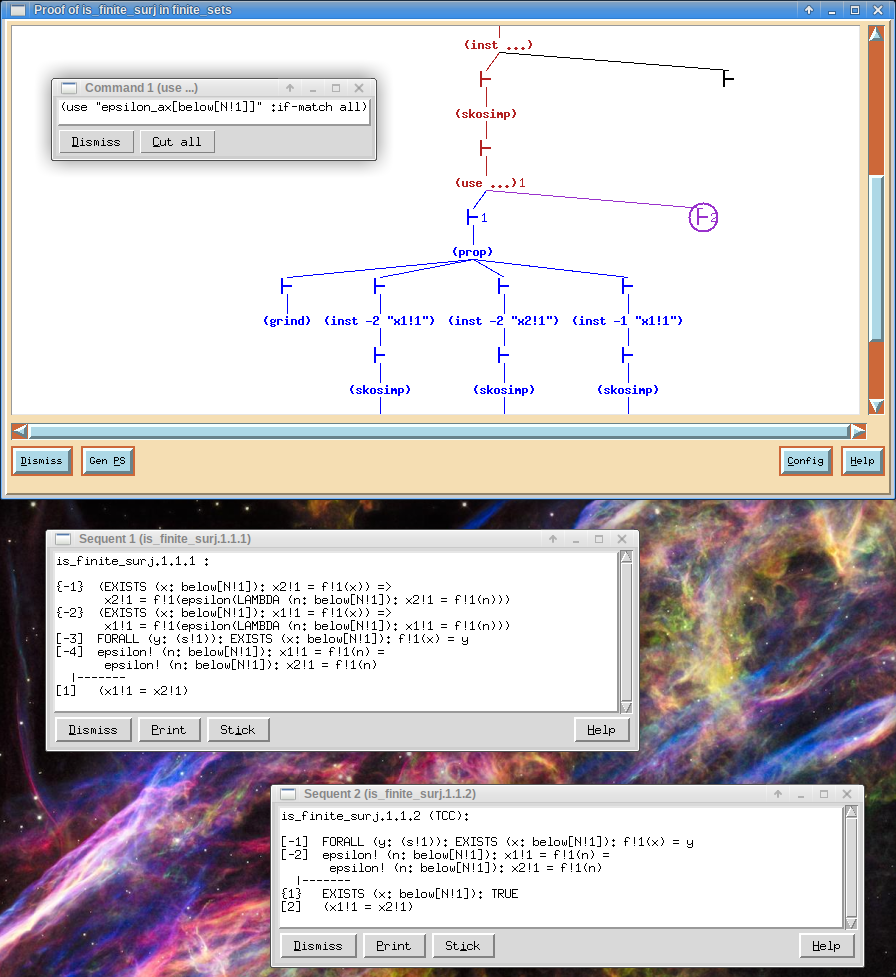
\includegraphics[width=\textwidth]{proofwindows.png}  
\caption{A Proof Display Example}\label{proofwindow}
\end{figure}

Colors are used to display status information about the proof.  These
colors may be specified using the X resource database (i.e., in your
\texttt{.Xresources} or \texttt{.Xdefaults} file).  Stipple patterns may
be specified instead of colors; a stipple pattern is specified as
\texttt{@file}, where \texttt{file} is either an absolute pathname of a
file in X bitmap format or the special bitmap name
\texttt{gray}.\footnote{If \texttt{file} is not an absolute path, it is
looked up in the \texttt{wish} subdirectory of the PVS directory, which
contains the \texttt{gray} bitmap.}

The current resources and their defaults are:

\begin{center}
\begin{tabular}{|lll|}\hline
  {\it Resource name} & {\it Color default} & {\it Monochrome default}%
     \\ \hline
  \texttt{pvs.windowbackground} & wheat & white \\
  \texttt{pvs.displaybackground} & white & white \\
  \texttt{pvs.displayforeground} & black & black \\
  \texttt{pvs.activedisplaybackground} & mediumslateblue & black \\
  \texttt{pvs.activedisplayforeground} & white & white \\
  \texttt{pvs.buttonbackground} & lightblue & white \\
  \texttt{pvs.buttonforeground} & black & black \\
  \texttt{pvs.activebuttonbackground} & steelblue & black \\
  \texttt{pvs.activebuttonforeground} & white & white \\
  \texttt{pvs.troughcolor} & sienna3 & black \\
  \texttt{pvs.currentColor} & DarkOrchid & black \\
  \texttt{pvs.circleCurrent} & yes & yes \\
  \texttt{pvs.tccColor} & green4 & black \\
  \texttt{pvs.doneColor} & blue & @gray \\
  \texttt{pvs.ancestorColor} & firebrick & black \\
  \texttt{pvs.abbrevLen} & 35 & 35 \\
  \texttt{pvs.displayfont} & \multicolumn{2}{l|}{lucidasanstypewriter-bold-12} \\
  \texttt{pvs.buttonfont} & \multicolumn{2}{l|}{lucidasanstypewriter-10} \\
  \texttt{pvs.proof.geometry} & \multicolumn{2}{l|}{\hspace*{.5in}\emph{none}} \\
  \texttt{pvs.theory-hierarchy.geometry} & \multicolumn{2}{l|}{\hspace*{.5in}\emph{none}} \\
  \texttt{pvs.prover-commands.geometry} & \multicolumn{2}{l|}{\hspace*{.5in}\emph{none}} \\
  \hline
\end{tabular}
\end{center}

The \texttt{foreground} color is used for things that aren't otherwise
specified below.  The \texttt{currentColor} is used for the current
sequent in the proof tree.  The \texttt{ancestorColor} is used for all
the ancestors of the current sequent, up to the root.  The
\texttt{doneColor} is used for sequents which have been proved.  The
\texttt{tccColor} is used for TCC's.  When \texttt{pvs.circle\-Current}
is set, the current sequent in the proof tree is circled.

Proof commands which are longer than \texttt{abbrevLen} characters are
abbreviated.

If the Emacs variable
\texttt{pvs-x-show-proofs}\index{pvs-x-show-proofs@\texttt{pvs-x-show-proofs}}
is not \texttt{NIL}, then \cmd{prove} automatically calls
\cmd{x-show-proof}.  This can be set in your
\texttt{.pvsemacs}\index{.pvsemacs@\texttt{.pvsemacs}} file.

The \cmd{x-theory-hierarchy} command prompts for a theory name and
displays the \texttt{IM\-PORTING} hierarchy rooted at that theory.  In a
complex hierarchy, it can be difficult to follow the lines; to make
this easier, when you move the mouse onto a theory identifier, all the
lines connecting that theory to other theories turn the
\texttt{highlight} color.  Clicking on a theory identifier will bring
up the theory in Emacs.  Figure~\ref{x-hierarchy} shows an example of the
theory hierarchy for the \texttt{finite\_sets} library, as produced from
clicking on the \texttt{Gen PS} button and selecting \texttt{portrait}.

\begin{figure}
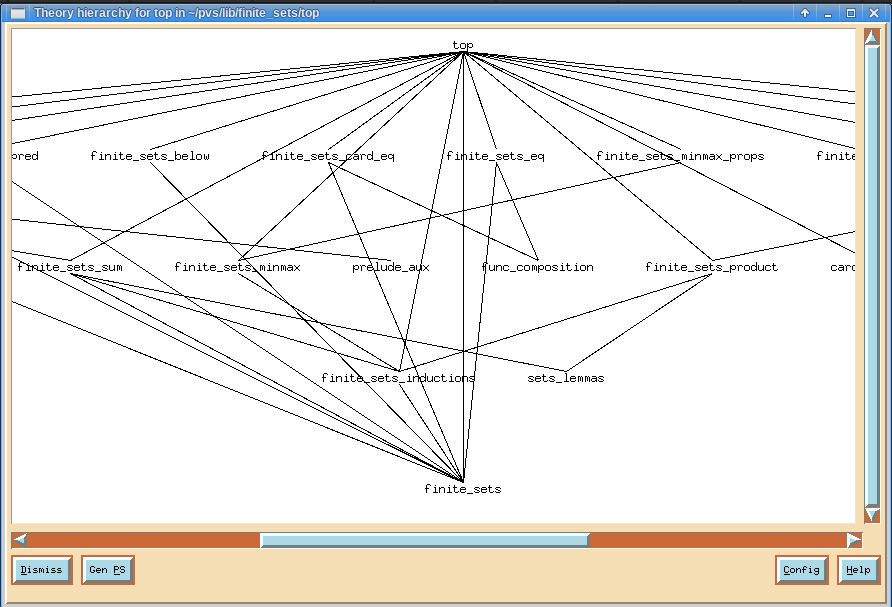
\includegraphics[width=\textwidth]{finite_sets_top_hier.png}
\caption{The Theory Hierarchy for the \texttt{finite\_sets} Library}\label{x-hierarchy}
\end{figure}


The remainder of this section applies to both \cmd{x-show-proof} and
\cmd{x-theory-hierarchy}.

The layout in the windows created by these commands can be manually
edited.  The editing commands are accessed by holding down the
\texttt{Control} key while pressing mouse buttons. In a proof window,
pressing \texttt{Control}-button~1 and dragging moves a whole proof
subtree, while \texttt{Control}-button~2 moves a single sequent.  In a
theory hierarchy window, \texttt{Control}-button~1 moves a theory.
(Note that most proof commands will do a relayout.)  Once the layout
is to your liking, the \texttt{Gen~PS} button will generate a
PostScript file which contains the contents of the window.  The
filename will be briefly displayed below the buttons.

The \texttt{Config} button will bring up a menu which will let you
customize the horizontal and vertical separations used by the
automatic layout for the current window.  These can also be customized
with the resource database.

\begin{center}
\begin{tabular}{|ll|}\hline
  {\it Resource name} & {\it Default} \\ \hline
  \texttt{pvs*proof*xSep} & 10 \\
  \texttt{pvs*proof*ySep} & 20 \\
  \texttt{pvs*th-hier*xSep} & 50 \\
  \texttt{pvs*th-hier*ySep} & 100 \\
  \hline
\end{tabular}
\end{center}


\section{Context Commands}

\begin{pvscmds}
\icmd{list-pvs-files} & \icmd{lf} & Display a list of PVS files in current context \\
\icmd{list-theories} & \icmd{lt} & Display a list of theories in current context \\
\icmd{change-context} & \icmd{cc} & Switch to a new context \\
\icmd{save-context} & \icmd{sc} & Save the current context \\
\icmd{pvs-remove-bin-files} & & Remove the \texttt{.bin} files of the current
context \\
\icmd{pvs-dont-write-bin-files} & & Inhibit writing or loading of
\texttt{.bin} files \\ 
\icmd{pvs-do-write-bin-files} & & Allows writing and loading of
\texttt{.bin} files (default) \\
\icmd{context-path} & \icmd{cp} & Display pathname of current context \\
\end{pvscmds}

The \cmd{list-pvs-files} and \cmd{list-theories} commands prompt for a
directory, default is to the current directory; if there is a PVS
context in the given directory, these commands list the PVS files or
theories in that context.  The resulting buffer is in a special mode,
which allows the file/theory to be viewed (by typing a ``\texttt{v}''),
selected (by typing a ``\texttt{s}'') or imported (by typing an ``{\tt
i}'').  A file or theory may only be selected if it is in the current
context, and may only be imported if it is not.  Importing a theory from
the list of theories will import the associated file.

The \cmd{change-context} command is similar to the ``\texttt{cd}'' command
in \unix; it saves the context (see below), and changes the working
directory to the specified one.  The \ibuf{PVS Welcome} buffer is then
displayed indicating the new directory.  If the requested directory does
not exist, and the Emacs you are running supports \texttt{make-directory},
then PVS offers to make a new one, including parent directories if necessary.
If the command fails for any reason, then the current context
stays the same.

The \cmd{save-context} command saves the current state of the session in
the context file \texttt{.pvscontext}.  In addition, any PVS files that
have been typechecked will generate a binary (\texttt{.bin}) file, unless
there is already a current one saved, or the \cmd{dont-write-bin-files}
command has been invoked.

Under normal circumstances, binary (\texttt{.bin}) files \index{.bin@\texttt{.bin}} corresponding to
the specification (\texttt{.pvs}) files are updated or created as needed.
These binary files contain type information, so that loading a binary file
has the same effect as typechecking the corresponding PVS file, but is
generally much faster.  The down side is that binary files take more disk
space.  If that is a problem then use the \cmd{pvs-dont-write-bin-files},
which neither loads nor creates binary files.  This can be added to your
\texttt{.pvsemacs}\index{.pvsemacs@\texttt{.pvsemacs}} file, by adding the
line
\begin{alltt}
  (pvs-dont-write-bin-files)
\end{alltt}
The \cmd{pvs-do-write-bin-files} undoes the effect of the
\cmd{pvs-dont-write-pvs-files}, and is not needed normally.  The
\cmd{pvs-remove-bin-files} command may be used to remove the binary files
that have been created.

The \cmd{context-path} command uses the minibuffer to display the
directory path associated with the current context.

\glossary{[directory path:] a file pathname containing sufficient
components to uniquely identify a directory}
\glossary{[context path:] a file pathname identifying the
directory which contains the context}

\section{Library Commands}

\begin{pvscmds}
\icmd{load-prelude-library} & & Extend the prelude from the specified context \\
\icmd{remove-prelude-library} & & Remove the specified context from the
prelude \\
\end{pvscmds}

The \cmd{load-prelude-library} command prompts for a context pathname
(\ie directory), and extends the prelude with all of the theories that
make up that context.  Note that the theories that make up the context are
defined by the \texttt{.pvscontext} file in the associated
directory---there may be specification files in the same directory that
are not a part of the context.  The files that make up the context are
typechecked if necessary, and internally the prelude is extended.  All of
the theories of the current context are untypechecked, as they may not
typecheck the same way in the extended prelude.  The PVS context is
updated to reflect that the prelude has been extended.  Thus the next time
this context is entered, the prelude will automatically be extended (by
typechecking the libraries if necessary).

This is just one of two means of gaining access to theories of a different
context (short of copying them).  For an alternative approach see the
language guide~\cite{PVS:language}.

The \cmd{remove-prelude-library} command removes the specified library
from the prelude.  It reverts all the theories of the current context to
untypechecked to guarantee that no theories depend on the removed library.
Note that the built-in prelude may not be removed this way.

\section{Browsing}

\begin{pvscmds}
\icmd{show-declaration} & \key{M-.} & Show declaration of symbol at cursor
\\
\icmd{goto-declaration} & \key{M-'} & Go to declaration of symbol at cursor \\
\icmd{find-declaration} & \key{M-,} & Search for declarations of given symbol \\
\icmd{whereis-declaration-used} & \key{M-;} & Search for declarations which reference identifier \\
\icmd{whereis-identifier-used} & \key{C-M-;} & Search for declarations which reference identifier \\
\icmd{list-declarations} & \key{M-:} & Produce list of declarations in import chain \\
\icmd{show-expanded-form} & \key{C-.} & Show expanded form of term
containing region\\
& & \emph{Arg:} also expand names from the prelude \\
\end{pvscmds}

These commands browse a specification consisting of several PVS files
and theories, providing information about where entities are declared
and used.  All of these commands browse the prelude as well as user
files.

The \cmd{show-declaration} command is used to determine the declaration
associated with the symbol or name at the cursor.  Positioning the cursor
on a name in the specification and typing \key{M-.} yields a pop-up
buffer displaying the declaration.  This command is useful to determine
the type of a name, or the resolution determined by the typechecker for an
overloaded name.  Note that when used on a record accessor it will
display the declaration of the record rather than just the record field.

The \cmd{goto-declaration} command goes to the declaration associated with
the symbol or name at the cursor.  It pops up a buffer containing the
theory associated with the declaration, and positions the cursor at the
declaration.

The \cmd{find-declaration} command takes a name and returns a list of all
the declarations with that name, the default name is the one under the
cursor. Each row in the display specifies the declaration name, its
kind/type, and the theory to which it belongs.  Declarations in this list
may be viewed by placing the cursor on the row of interest and typing
``\texttt{v}.''  Typing ``\texttt{s}'' will read in the associated file
and position the cursor at the declaration.  A ``\texttt{q}'' quits and
removes the declaration buffer.

The \cmd{whereis-declaration-used} command generates a list of
declarations which reference the entity denoted by a given identifier.
The related \cmd{whereis\-identifier-used} command generates a list of all
references to a \emph{textually identical} identifier, which may or may
not result from the same declaration, due to overloading and multiple
declarations.  The \cmd{list-declarations} command generates a listing of
all the declarations in the import chain of the specified theory.  For all
of these commands, the resulting buffer behaves exactly as described for
\icmd{find-declaration}.

The \cmd{show-expanded-form} command displays the expanded form of the
term containing the region in the \texttt{Expanded Form} buffer.  Each
variable, constant and operator is expanded to its full name including the
theory name and its parameters, unless they are from the current theory or
the prelude.  With an argument, prelude names are also expanded.  If the
region is not defined, the current cursor location is used instead.

%\memo{How about a \LaTeX\ version?}

\section{Theory Status}

\begin{pvscmds}
\icmd{status-theory} & \icmd{stt}, \key{C-c C-s t} & Status of specified theory (parsed, etc.) \\
\icmd{status-pvs-file} & \icmd{stf}, \key{C-c C-s f} & Status of theories of current file \\
\icmd{status-importchain} & \icmd{sti}, \key{C-c C-s i}  & Status of theories in import chain of theory \\
\icmd{status-importbychain} & \icmd{stb}, \key{C-c C-s b} & Status of
theories in import by chain \\
\end{pvscmds}

These commands provide information regarding the status of the
specified theories.  The status information for a theory indicates whether
it is parsed or typechecked, and provides the number of formulas, the
number proved, the number of TCCs generated, and the number of TCCs
proved.  Note that the number of formulas does not include the TCCs.

The number of theory warnings and messages is also displayed.  See the
\cmd{show-theory-warnings} and \cmd{show-theory-messages} on
page~\pageref{tc-info} for more information on these commands.

The \cmd{status-theory} command provides the status of the specified
theory in the mini\-buffer.  The \cmd{status-pvs-file},
\cmd{status-importchain}, and \cmd{status\-importbychain} commands display
the information in the \ibuf{PVS Status} buffer with a line for each
theory.  Using any of these commands on the \texttt{sum} theory yields
{\small
\begin{alltt}
sum is typechecked: 1 formula, 1 proved; 2 TCCs, 2 proved; 0 warnings; 0 msgs
\end{alltt}}
The \cmd{show-theory-warnings} and \cmd{show-theory-messages}
(page~\pageref{tc-info}) may be used to see any warnings or messages.

The \cmd{status-importchain} and \cmd{status-importbychain} commands
display the \texttt{IM\-PORT\-ING} chains of the specified theory, indented to
indicate the tree structure.  The \cmd{status-importchain} command works
recursively down the \texttt{IMPORTING}s, displaying the status of each
theory unless it has been displayed earlier in the buffer.  The
\cmd{status-importbychain} works in the opposite direction.


\section{Proof Status}
\label{proof-status}

\begin{pvscmds}
\icmd{status-proof} & \icmd{sp}, \key{C-c C-s p} & Status of formula at cursor \\
\icmd{status-proof-theory} & \icmd{spt} & Status of formulas in theory \\
 & & \emph{Arg:} provide timing information \\
\icmd{status-proof-pvs-file} & \icmd{spf} & Status of formulas in PVS file \\
 & & \emph{Arg:} provide timing information \\
\icmd{status-proof-importchain} & \icmd{spi} & Status of formulas on importchain \\
 & & \emph{Arg:} provide timing information \\
\icmd{status-proofchain} & \icmd{spc} & Proofchain of formula at cursor \\
\icmd{status-proofchain-theory} & \icmd{spct} & Proofchain of
specified theory \\
\icmd{status-proofchain-pvs-file} & \icmd{spcf} & Proofchain of current file \\
\icmd{status-proofchain-importchain} & \icmd{spci} & Proofchain of importchain \\
\end{pvscmds}

These commands provide the status of the proofs of the indicated formulas.
The \cmd{status-proof} command uses the minibuffer to display the proof
status of the formula at the cursor.  The status can be one of
\texttt{proved}, \texttt{untried}, \texttt{unfinished}, or
\texttt{unchecked}.  Untried means that the proof has not yet been
attempted.  Unfinished means that the proof has been attempted,
but is not complete.  Unchecked means that the proof was successful at one
point, but that some changes have been made that may invalidate the proof.

The commands \cmd{status-proof-theory}, \cmd{status-proof-pvs-file}, and
\cmd{status\-proof-importchain} use the \ibuf{PVS Status} buffer
to display the proof status for all of the formulas within the theory, PVS
file, or the import chain respectively.  With an argument, these commands
display timing information as well.

The \cmd{status-proofchain} command provides a proof chain analysis of the
formula at the cursor and displays it in the \ibuf{PVS Status} buffer.
The proof chain analysis indicates whether the formula has been proved,
and analyses the formulas used in the proof to insure that the proof is
complete; lemmas used in the proof are proved and sound, \ie\ there are no
circularities (for example, using lemma $\mathcal{A}$ to prove
$\mathcal{B}$ and vice-versa).  Because judgements are used implicitly,
they may be included in the analysis even if they are not actually used.

The commands \cmd{status-proofchain-theory},
\icmd{status-proofchain-pvs-file}, and \newline
\icmd{status-proofchain-importchain} provide the proof chain analysis for
each formula of the theory, PVS file, and import chain of the specified
theory, respectively, in the \ibuf{PVS Status} buffer.

\section{Environment Commands}

\begin{pvscmds}
\icmd{whereis-pvs} & & Display the root PVS directory \\
\icmd{pvs-version} & & Display current version of PVS and underlying \lisp \\
\icmd{pvs-mode} & & Put current buffer in PVS mode \\
\icmd{pvs-log} & & Display the \ibuf{PVS Log} buffer \\
\icmd{status-display} & & Display the \ibuf{PVS Status} buffer \\
\icmd{pvs-status} & & Find out if PVS is busy \\
\icmd{pvs} & & Start the PVS process \\
\icmd{pvs-load-patches} & & Load new PVS patches \\
\end{pvscmds}

The \cmd{whereis-pvs} command is used to determine the directory where the
PVS system resides.  This is useful for finding the example specifications
and files that are part of the PVS distribution.

The \cmd{pvs-version} command displays the current version of PVS\@.

The \cmd{pvs-mode} command puts the current buffer in PVS mode.  This
command is not normally needed; buffers with a \ibuf{.pvs}
extension and buffers created by PVS are automatically put in the
proper mode.

Most of the messages that appear in the minibuffer are kept in the
\ibuf{PVS Log} buffer, stamped with the time.  The \cmd{pvs-log} command
simply pops up the \ibuf{PVS Log} buffer so that you may view it.

The \cmd{status-display} command simply displays the \ibuf{PVS Status}
buffer.  This is the buffer used for most of the status commands.

The \cmd{pvs} command is what is used to actually start PVS after the
Emacs files have all been loaded.  It is provided as a user command
because there are times when the PVS lisp subprocess has been killed and
you wish to start up that process while keeping the same Emacs session.

The \cmd{pvs-load-patches} command reloads the patches.  This is useful
when new patches have been installed, and you wish to load them without
exiting the system and starting up again.


\section{Interrupting PVS}

\begin{pvscmds}
\icmd{pvs-status} & & Find out if Lisp is busy \\
\icmd{pvs-interrupt-subjob} & \key{C-c C-c} & Interrupt PVS (lisp)
  process \\
\icmd{reset-pvs} & \key{C-z C-g} & Abort PVS and resynchronize \\
\end{pvscmds}

Many PVS commands run in the background, allowing other editing
activities to proceed concurrently.  The effect of issuing new commands
while another command is running depends on the command: 
background commands placed on the command queue.  Other (nonbackground
commands) interrupt the currently running command, execute, and return
control to the interrupted command.  The Emacs status line indicates
the abbreviation of the command that is currently running, if any, or {\tt
ready}.  The \cmd{pvs-status} command provides information
about both the currently running command and the command queue.

To interrupt PVS for any reason, the following procedure is recommended.
First, if the keyboard is not responding, type the built-in Emacs
command \cmd{keyboard-quit} (\key{C-g}); it may need to be struck a few
times before there is any response---usually a beep and \texttt{Quit}
appears in the minibuffer.  This command interrupts Emacs, but has no
effect on any PVS commands that are still running.  After Emacs responds
go to the end of the \texttt{*pvs*} buffer, and type \key{C-c C-c}.  If
Lisp is able to respond, you should see the message
{\small\small
\begin{alltt}
Error: Received signal number 2 (Keyboard interrupt)
  [condition type: INTERRUPT-SIGNAL]

Restart actions (select using :continue):
 0: continue computation
 1: Return to Top Level (an "abort" restart)
[1c] PVS(22):
\end{alltt}}
You can then type \texttt{:continue 0} to keep going as it was never
interrupted, \texttt{(restore)} if you are in the middle of an ongoing
proof and want to continue from the state prior to the last \emph{atomic}
prover command (see the prover guide~\cite{PVS:prover}), or
\texttt{:continue 1} or \texttt{:reset} to abort to the top level.

The Lisp process may not be able to respond to the interrupt right away,
especially if it has started garbage collection.  If you really want to
interrupt it, type more \key{C-c C-c} interrupts; after about six of them
it is supposed to respond regardless.  This is not recommended in general
as it can leave the Lisp process in an unstable state.  Unfortunately, we
have seen Allegro Common Lisp get into a state where it is completely
unresponsive, even after several interrupts and waiting for hours for a
response.  This is rare, but if it happens the only recourse is to kill
the process and start up a new PVS session.  See below for how to do this
while allowing Emacs to continue.

The \cmd{reset-pvs} command aborts any ongoing activity in PVS; its
effects depend on whether it is issued from the \ibuf{*pvs*} buffer or
from some other buffer.  In the former case, \cmd{reset-pvs} simply
interrupts PVS as if you typed \key{C-c C-c}, as described above.  If
\cmd{reset-pvs} is issued somewhere other than the \ibuf{*pvs*} buffer,
you are asked whether to reset PVS in case the command was typed
accidentally; if not, the current command is aborted and the command queue
is emptied.

If you wish to kill the PVS Lisp process, while keeping your current Emacs
session, simply go to the \texttt{*pvs*} buffer and kill it
\icmd{kill-buffer} \key{C-x k}, then run \icmd{pvs} and the PVS Lisp
process will restart.  All your other Emacs buffers are unaffected by
this.
